\documentclass{beamer}
\usepackage[swedish]{babel}
\usepackage[utf8]{inputenc}
\usepackage[utf8]{inputenc}
\usepackage{amsmath}
\usepackage{amssymb}
\usepackage{amsthm}
\usepackage{graphicx}

\uselanguage{swedish}
\languagepath{swedish}
\deftranslation[to=swedish]{Theorem}{Sats}
\deftranslation[to=swedish]{theorem}{sats}
\deftranslation[to=swedish]{Corollary}{Följdsats}
\deftranslation[to=swedish]{corollary}{följdsats}
\deftranslation[to=swedish]{Example}{Exempel}
\deftranslation[to=swedish]{example}{exempel}




\usetheme{Warsaw}

\title[Algoritmer och komplexitet inom algebraisk geometri]{
	Algoritmer och komplexitet inom \\
	kommutativ algebra \& algebraisk geometri \\[10pt]
	\large Omparametrisering av kurvor, semigrupper, \\
	implicit notation \& multiplicitetsföljder}

\author[Peter Waher]{Peter Waher \\[5pt]
	\texttt{peterwaher@hotmail.com}\\
	\texttt{https://github.com/PeterWaher/Algebraiska\_kurvor}\\[5pt]
	$\mathfrak{L}_2$}

\begin{document}

\begin{frame}
	\titlepage
\end{frame}

\begin{frame}
	\frametitle{Outline}
	\tableofcontents[pausesections]
\end{frame}





\section{Plana algebraiska kurvor}

\begin{frame}
	\frametitle{Plana algebraiska kurvor}
	\begin{center}
		\Large Plana algebraiska kurvor
		
		Introduktion
	\end{center}
\end{frame}

\subsection{Introduktion - kurvor}

\begin{frame}
\frametitle{Vad är en plan kurva?}
\begin{Definition}
	En \textbf{plan kurva} $C$ är en delmängd i $\mathbb{C}^2$ sådan att det finns två kontinuerliga funktioner $f : \mathbb{C} \rightarrow \mathbb{C}$ och 
	$g : \mathbb{C} \rightarrow \mathbb{C}$ sådana att $C = \left\{\left(f(t), g(t)\right) : t \in \mathbb{C}\right\}$. $(f, g)$ är en \textbf{parametrisering} av $C$. Om $C$ kan parametriseras av två analytiska funktioner $f$ och $g$ kallas $C$ \textbf{analytisk}. Om den kan parametriseras av två polynom kallas $C$ för \textbf{algebraisk}. Om den kan parametriseras av två formella potensserier kallas $C$ \textbf{algebroid}.
\end{Definition}
\end{frame}

\begin{frame}
	\frametitle{Kurvor i det Euklidiska planet}
	Traditionellt har man ofta studerat plana kurvor i det \emph{Euklidiska planet}. I detta fall är kurvan parametriserad av reellvärda funktioner $f : \mathbb{R} \rightarrow \mathbb{R}$ och 
	$g : \mathbb{R} \rightarrow \mathbb{R}$.
	
  	\begin{example}
		\begin{columns}[onlytextwidth]
			\begin{column}{0.55\textwidth}
				\[C(t)=(t^2,t^3+t^7)\]\\[10pt]
				\scriptsize Not: För att förenkla notationen kan vi identifiera kurvan $C$ med en viss parametrisering $(f, g)$, även om parametriseringen inte är unik. Detta görs enklast genom att identifiera kurvan med funktionen $C : \mathbb{C} \rightarrow \mathbb{C}^2$, $C(t) = \left(f(t), g(t)\right)$. Notera dock att kurvan som sådan och en av dess parametriseringar är två olika objekt.
			\end{column}
			\begin{column}{0.45\textwidth}
				\begin{center}
				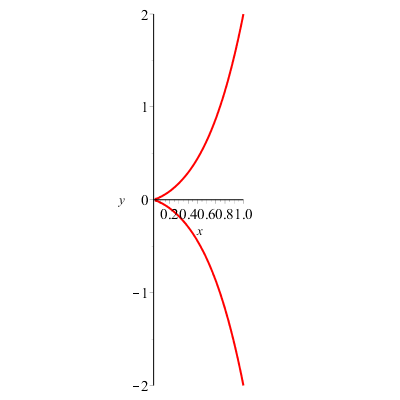
\includegraphics[scale=0.3]{Export/blowupex1_1.png}
				\end{center}
			\end{column}
		\end{columns}
  	\end{example}
\end{frame}


\begin{frame}
	\frametitle{Förenklingar}
	Förenklingar vi kan göra om vi studerar en plan kurva lokalt:
	
	\begin{enumerate}
		\item<1-> Tillräckligt att studera \emph{algebraiska} kurvor:
		\begin{enumerate}
			\item<2-> Analytiska funktioner kan skrivas som formella potensserier kring den punkt vi studerar.
			\item<3-> Formella potensserier kan approximeras av polynom med önskad noggrannhet.
		\end{enumerate}
		\item<4-> Kurvan går genom \emph{origo}: $C(0) = \mathbf{0}$
	\end{enumerate}
\end{frame}

\begin{frame}
	\frametitle{Reguljära och singulära kurvor}
\begin{Definition}
	Om en kurva $C$ har en parametrisering $(f, g)$ sådan att $f'(0) \neq 0$ eller $g'(0) \neq 0$ kallas kurvan \textbf{reguljär}. Annars kallas kurvan \textbf{singulär}.
\end{Definition}

\vspace{20pt}
\scriptsize Not: Bara för att $f'(0) = 0$ och $g'(0) = 0$ i en parametrisering $(f, g)$ av en kurva $C$, betyder inte det att kurvan är singulär. Det kan ju finnas en parametrisering av samma kurva där någon av derivatorna är nollskilda. Exempelvis är $(t^3, t^3)$ och $(t, t)$ två olika parametriseringar av samma kurva. I det första exemplet är derivatorna $0$ i origo medan de i det andra exemplet båda är nollskilda.
\end{frame}

\begin{frame}
	\frametitle{Ordning och grad}
\begin{Definition}
	\textbf{Ordningen} av ett polynom eller en potensserie $f(t) =
	\sum a_i t^i \neq 0$ är det minsta heltalet $k$ sådant att koefficienten $a_k$ är nollskild, och skrivs $\mathbf{o}(f)$. \textbf{Graden} for motsvarande polynom är det största heltalet $k$ sådant att koefficienten $a_k$ inte är noll, och skrivs $\deg(f)$.
\end{Definition}
\end{frame}

\subsection{Omparametrisering}

\begin{frame}
	\frametitle{Plana algebraiska kurvor}
	\begin{center}
		\Large Plana algebraiska kurvor
		
		Omparametrisering
	\end{center}
\end{frame}

\begin{frame}
	\frametitle{Varför omparametrisera?}
	\begin{enumerate}
		\item För utritande av kurvor spelar parametriseringen inte så stor roll.
		
		\item Vill man beräkna $y(x) = g(f^{-1}(x))$ eller $x(y) = f(g^{-1}(y))$, står man genast inför en mängd problem.
	\end{enumerate}
\end{frame}

\begin{frame}
	\frametitle{Omparametrisering av kurvor}
\begin{Theorem}
	Om $C = C(t) = \left(f(t), g(t)\right)$ är en komplex analytisk, algebroid eller algebraisk kurva, samt att $f(0) = g(0) = 0$, kan kurvan $C$ omparametriseras på formen $C^*(t) = \left(\pm t^n, g^*(t)\right)$ eller på formen $C^*(t) = \left(f^*(t), \pm t^n \right)$ i ett område kring $t = 0$, där $f(t)$ och $g(t)$ är formella potensserier. Dessutom gäller att $\mathbf{o}\left(f^*\right) \geq n$ eller att $\mathbf{o}\left(g^*\right) \geq n$. Om $f(t)$ och $g(t)$ är reellvärda, kan också omparametriseringen göras reellvärd.
\end{Theorem}

\vspace{20pt}
\scriptsize Not: Från \emph{Weierstrass Preparation Theorem} kan man få att en sådan omparametrisering existerar. Dock presenteras inte en metod över hur en sådan omparametrisering kan tas fram.
\end{frame}

\begin{frame}
	\frametitle{Översikt bevis}
	Beviset av satsen går igenom följande steg:
	
	\begin{enumerate}
		\item<1-> Vi skapar en omparametrisering via komposition med $\phi(t)$:
		\[C^*(t) = (f^*(t), g^*(t)) = (f(\phi(t)), g(\phi(t)))\]
		
		\item<2-> Vi väljer $\phi(t)$ sådan att:
		\begin{enumerate}
			\item<3-> Analytisk kring $t = 0$.
			
			\item<4-> $\phi(0)=0$
			
			\item<5-> $\mathbf{o}(\phi)=1 \Longrightarrow \mathbf{o}(f(\phi))=\mathbf{o}(f) \wedge \mathbf{o}(g(\phi))=\mathbf{o}(g)$
			
			\item<6-> $\phi(t), f(t), g(t)$ reellvärda $\Longrightarrow$ $C^*(t)$ reellvärd.
			
		\end{enumerate}
		
		\item<7-> Med början i $a_1$ (som har $n$ lösningar), löses koefficienterna $a_i$ ut ur $\phi(t)=\sum_{k=1}^{\infty}a_k t^k$ för att uppfylla ovanstående.
		
		\item<8-> Finns precis en lösning i det generella fallet som uppfyller ovanstående, samt satsens, krav.
		\qed
	\end{enumerate}
\end{frame}

\begin{frame}
	\frametitle{\texttt{Reparametrize()}}

\begin{semiverbatim}
Reparametrize := proc(x, y, Variable, t0 , MaxDegree,

\qquad Branch, AllowNegation)
\end{semiverbatim}
	
	\begin{enumerate}
		\item<1-> Algoritm som omparametriserar en algebraisk kurva med given noggrannhet.
		
		\item<2-> Maple-kod finns i \texttt{https://github.com/PeterWaher/\\
			\qquad Algebraiska\_kurvor/blob/master/kurvor.mw}
		
		\item<3-> Text-version finns i
		\texttt{https://github.com/PeterWaher/\\
			\qquad Algebraiska\_kurvor/blob/master/Functions/\\
			\qquad Reparametrize.txt} 
	\end{enumerate}
\end{frame}




\begin{frame}
	\frametitle{Reparametrize - exempel 1 (1/4)}
	
  	\begin{example}
  		Kurvan $(t^2+t^3,t^5+t^6)$ har en singularitet i $t = 0$. Dessutom passerar kurvan genom origo då $t = -1$.
  		
		\begin{center}
			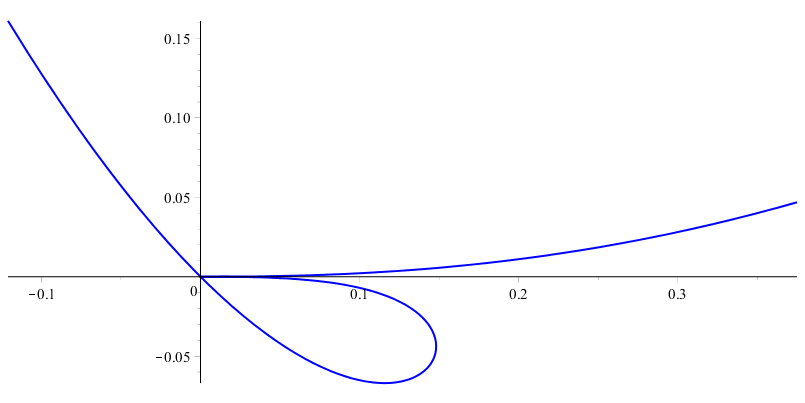
\includegraphics[scale=0.35]{Export/kurvorplot2d1_0.png}
		\end{center}
  	\end{example}
\end{frame}
  		
\begin{frame}
	\frametitle{Reparametrize - exempel 1 (2/4)}
	
	\begin{example}
  		Först ber vi Maple att parametrisera om kurvan kring $t = 0$:
  		
		\begin{semiverbatim}
		> Reparametrize(t\^{}3+t\^{}2,t\^{}6+t\^{}5,t,0,10,0,false);
		
		
		Elapsed Time: 0.016 s.
		\end{semiverbatim}
				 
		 \[\left[{t}^{2},{t}^{5}-3/2\,{t}^{6}+{\frac {21\,{t}^{7}}{8}}-5\,{t}^{8}+{\frac {1287\,{t}^{9}}{128}}-21\,{t}^{10}\right]\]
  	\end{example}
\end{frame}

\begin{frame}
	\frametitle{Reparametrize - exempel 1 (3/4)}
	
	\begin{example}
		Därefter vill vi ha en omparametrisering kring $t = -1$:

\begin{semiverbatim}
> Reparametrize(t\^{}3+t\^{}2, t\^{}6+t\^{}5, t, -1, 10,

\qquad 0, false);


Elapsed Time: 0.016 s.
\end{semiverbatim}		
		\[\left[t,163438\,{t}^{10}+29070\,{t}^{9}+5304\,{t}^{8}+1001\,{t}^{7}+198\,{t}^{6}+42\,{t}^{5}+\right.\]
		\[\left.+10\,{t}^{4}+3\,{t}^{3}+3\,{t}^{2}-t\right]\]
	\end{example}
\end{frame}

\begin{frame}
	\frametitle{Reparametrize - exempel 1 (4/4)}
	
	\begin{example}
	Nedan kurvan $C(t)=(t^2+t^3,t^5+t^6)$, med omparametriseringarna kring $t=0$ och $t=-1$.
	
		\begin{center}
			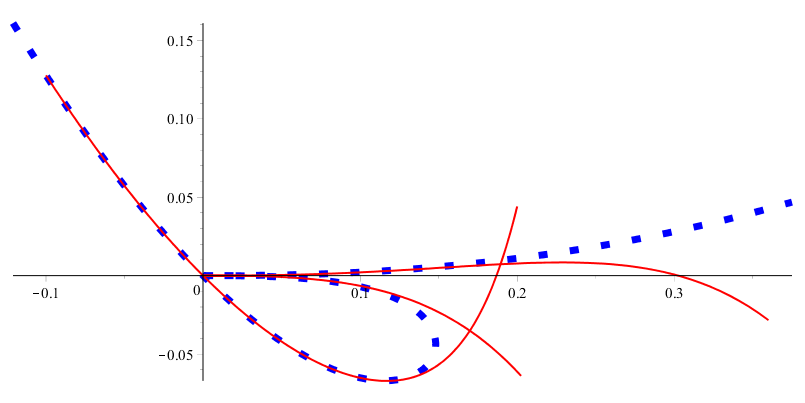
\includegraphics[scale=0.35]{Export/kurvorplot2d1.png}
		\end{center}
	\end{example}
\end{frame}






\begin{frame}
	\frametitle{Reparametrize - exempel 2 (1/6)}
	
	\begin{example}
		Ellipsen $\left(3 \sin(t), 2 \cos(t)\right)$ är reguljär, men vi kan parametrisera om kurvan ändå för att illustrera axelbyte. 
  		
  		\begin{center}
  			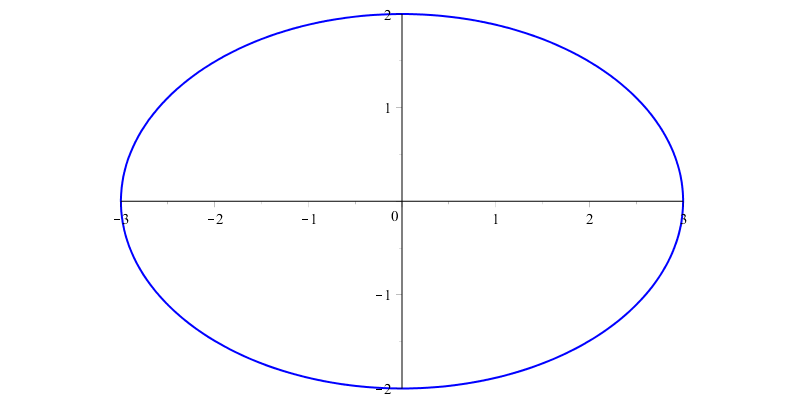
\includegraphics[scale=0.35]{Export/kurvorplot2d2_0.png}
  		\end{center}
  	\end{example}
  \end{frame}
  
  \begin{frame}
  	\frametitle{Reparametrize - exempel 2 (2/6)}
  	
  	\begin{example}
		Första omparametriseringen gör vi kring $t=0$:

		\begin{semiverbatim}
			> Reparametrize(3*sin(t),2*cos(t),t,0,10,0,false);
			
			
			Elapsed Time: 0.015 s.
		\end{semiverbatim}
		
		\[\left[t,2-1/9\,{t}^{2}-{\frac {{t}^{4}}{324}}-{\frac {{t}^{6}}{5832}}-{\frac {5\,{t}^{8}}{419904}}-{\frac {7\,{t}^{10}}{7558272}}\right]\]
	\end{example}
\end{frame}

\begin{frame}
	\frametitle{Reparametrize - exempel 2 (3/6)}
	
	\begin{example}
		Andra omparametriseringen gör vi kring $t=\pi$:
		
		\begin{semiverbatim}
			> Reparametrize(3*sin(t),2*cos(t),t,Pi,10,0,false);
			
			
			Elapsed Time: 0.016 s.
		\end{semiverbatim}
		
		\[\left[t,-2+1/9\,{t}^{2}+{\frac {{t}^{4}}{324}}+{\frac {{t}^{6}}{5832}}+{\frac {5\,{t}^{8}}{419904}}+{\frac {7\,{t}^{10}}{7558272}}\right]\]
	\end{example}
\end{frame}

\begin{frame}
	\frametitle{Reparametrize - exempel 2 (4/6)}
	
	\begin{example}
		Tredje omparametriseringen gör vi kring $t=\frac{\pi}{2}$. Notera hur omparametriseringarna skiljer från $t=0$ och $t=\pi$, jämfört med $t=\pm \frac{\pi}{2}:$
		
		\begin{semiverbatim}
			> Reparametrize(3*sin(t),2*cos(t),t,(1/2)*Pi,

			\qquad 10,0,false);
			
			
			Elapsed Time: 0.016 s.
		\end{semiverbatim}
		
		\[\left[3-3/8\,{t}^{2}-{\frac {3\,{t}^{4}}{128}}-{\frac {3\,{t}^{6}}{1024}}-{\frac {15\,{t}^{8}}{32768}}-{\frac {21\,{t}^{10}}{262144}},t\right]\]
	\end{example}
\end{frame}

\begin{frame}
	\frametitle{Reparametrize - exempel 2 (5/6)}
	
	\begin{example}
		Fjärde omparametriseringen gör vi kring $t=-\frac{\pi}{2}$:
		
		\begin{semiverbatim}
			> Reparametrize(3*sin(t),2*cos(t),t,-(1/2)*Pi,
			
			\qquad 10,0,false);
			
			
			Elapsed Time: 0.015 s.
		\end{semiverbatim}
		
		\[\left[-3+3/8\,{t}^{2}+{\frac {3\,{t}^{4}}{128}}+{\frac {3\,{t}^{6}}{1024}}+{\frac {15\,{t}^{8}}{32768}}+{\frac {21\,{t}^{10}}{262144}},t\right]\]
	\end{example}
\end{frame}

\begin{frame}
	\frametitle{Reparametrize - exempel 2 (6/6)}
	
	\begin{example}
		Nedan kurvan $C(t)=(3\sin(t),2\cos(t))$, med de fyra omparametriseringarna kring $t=0$, $t=\pi$ och $t=\pm \frac{\pi}{2}$:
		
		\begin{center}
			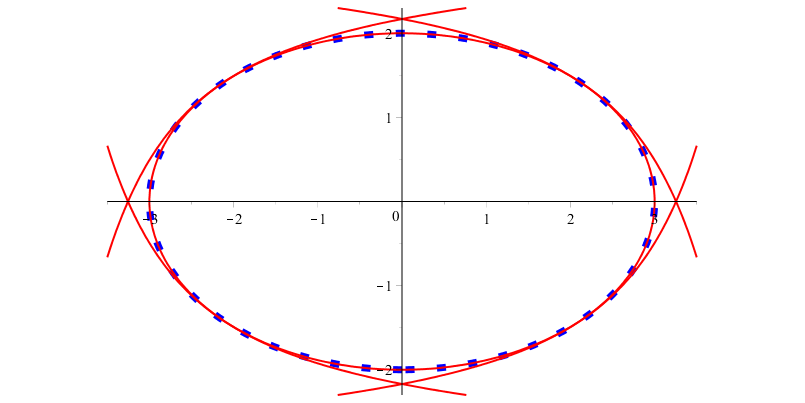
\includegraphics[scale=0.35]{Export/kurvorplot2d2.png}
		\end{center}
	\end{example}
\end{frame}






\begin{frame}
	\frametitle{Reparametrize - exempel 3 (1/5)}
	
	\begin{example}
		Kurvan $\left(t^3(t - 1)^3(t + 1)^3,t^5(t - 1)^2(t + 1)^2\right)$ har singulariteter i $t = 0, 1, -1$ av ordningar 2, 1, 1 respektive.
  		
  		\begin{center}
  			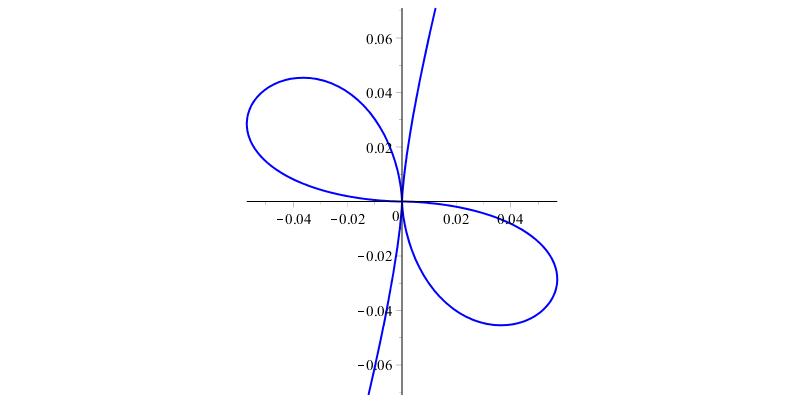
\includegraphics[scale=0.35]{Export/kurvorplot2d3_0.png}
  		\end{center}
  	\end{example}
  \end{frame}
  
  \begin{frame}
  	\frametitle{Reparametrize - exempel 3 (2/5)}
  	
  	\begin{example}
		Vi analyserar hur omparametriseringarna uppför sig i dessa tre singulariteter. Första omparametriseringen gör vi kring $t=0$:

		\begin{semiverbatim}
			> Reparametrize(t\^{}3*(t-1)\^{}3*(t+1)\^{}3,

			\qquad t\^{}5*(t-1)\^{}2*(t+1)\^{}2,t,0,15,0, false);
			
			
			Elapsed Time: 0.031 s.
		\end{semiverbatim}
		
		\[\left[{t}^{3},-1428\,{t}^{15}-273\,{t}^{13}-55\,{t}^{11}-12\,{t}^{9}-3\,{t}^{7}-{t}^{5}\right]\]
	\end{example}
\end{frame}

\begin{frame}
	\frametitle{Reparametrize - exempel 3 (3/5)}
	
	\begin{example}
		Därefter kring $t=1$:
		
		\begin{semiverbatim}
			> Reparametrize(t\^{}3*(t-1)\^{}3*(t+1)\^{}3,
			
			\qquad t\^{}5*(t-1)\^{}2*(t+1)\^{}2,t,1,15,0,false);
			
			
			Elapsed Time: 0.063 s.
		\end{semiverbatim}
		
		\[\begin{array}{l}
		\left[1/2\, \sqrt{4}{t}^{3}-9/4\,{t}^{4}+{\frac {207\, \sqrt{4}{t}^{5}}{64}}-21\,{t}^{6}+{\frac {150183\, \sqrt{4}{t}^{7}}{4096}}\right. \\
		\mbox{}-{\frac {137655\,{t}^{8}}{512}}+{\frac {66893079\, \sqrt{4}{t}^{9}}{131072}}-3978\,{t}^{10}+{\frac {132735945771\, \sqrt{4}{t}^{11}}{16777216}}\\
		\mbox{}-{\frac {8385901667\,{t}^{12}}{131072}}+{\frac {70379121262905\, \sqrt{4}{t}^{13}}{536870912}}\\
		\left.\mbox{}-{\frac {4345965\,{t}^{14}}{4}}+{\frac {78087826643607459\, \sqrt{4}{t}^{15}}{34359738368}},{t}^{2}\right]
		\end{array}\]
	\end{example}
\end{frame}

\begin{frame}
	\frametitle{Reparametrize - exempel 3 (4/5)}
	
	\begin{example}
		Och sist kring $t=-1$:
		
		\begin{semiverbatim}
			> Reparametrize(t\^{}3*(t-1)\^{}3*(t+1)\^{}3,
			
			\qquad t\^{}5*(t-1)\^{}2*(t+1)\^{}2,t,-1,15,0,true);
			
			
			Elapsed Time: 0.047 s.
		\end{semiverbatim}
		
		\[\begin{array}{l}
		\left[1/2\, \sqrt{4}{t}^{3}+9/4\,{t}^{4}+{\frac {207\, \sqrt{4}{t}^{5}}{64}}+21\,{t}^{6}+{\frac {150183\, \sqrt{4}{t}^{7}}{4096}}\right.\\
		\mbox{}+{\frac {137655\,{t}^{8}}{512}}+{\frac {66893079\, \sqrt{4}{t}^{9}}{131072}}+3978\,{t}^{10}+{\frac {132735945771\, \sqrt{4}{t}^{11}}{16777216}}\\
		\mbox{}+{\frac {8385901667\,{t}^{12}}{131072}}+{\frac {70379121262905\, \sqrt{4}{t}^{13}}{536870912}}\\
		\left.\mbox{}+{\frac {4345965\,{t}^{14}}{4}}+{\frac {78087826643607459\, \sqrt{4}{t}^{15}}{34359738368}},-{t}^{2}\right]
		\end{array}\]
	\end{example}
\end{frame}

\begin{frame}
	\frametitle{Reparametrize - exempel 3 (5/5)}
	
	\begin{example}
		Ritar vi sedan ut originalparametriseringen av kurvan tillsammans med de tre omparametriseringarna får vi följande intressanta bild:

		\begin{center}
			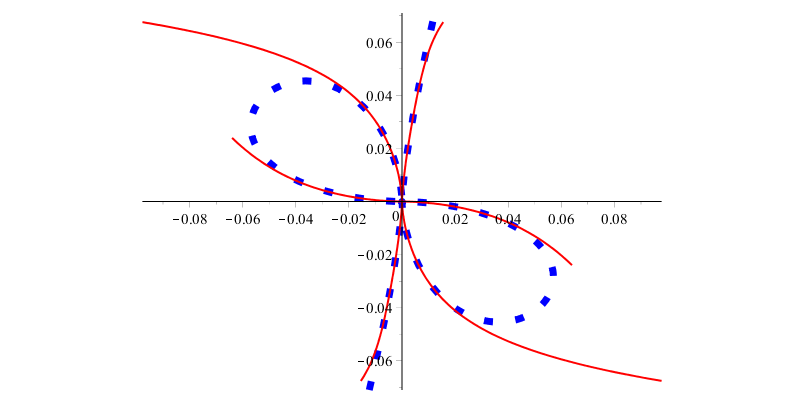
\includegraphics[scale=0.35]{Export/kurvorplot2d3.png}
		\end{center}
	\end{example}
\end{frame}








\section{Semigrupper}

\subsection{Introduktion - semigrupper}

\begin{frame}
	\frametitle{Plana algebraiska kurvor}
	\begin{center}
		\Large Semigrupper
		
		Introduktion
	\end{center}
\end{frame}

\begin{frame}
	\frametitle{Modulär aritmetik}
\begin{Definition}
	Heltalen $m \in \mathbb{Z}^+$ och $n \in \mathbb{Z}^+$ sägs vara \textbf{relativt prima} om $m \geq 2$, $n \geq 2$ samt $p \mid m \wedge p \mid n \Longrightarrow p = 1$.
\end{Definition}
\uncover<2->{\begin{Lemma}
	Om $m$ och $n$ är relativt prima och $0 < a < m$ gäller att $[a \cdot n]_m \neq 0$.
	\end{Lemma}}
\uncover<3->{\begin{Lemma}
		Om $m$ och $n$ är relativt prima och $0 < a, b < m$ gäller:
		\[[a \cdot n]_m = [b \cdot n]_m \Longleftrightarrow a = b\]
	\end{Lemma}}
\end{frame}

\begin{frame}
	\frametitle{Semigrupper}
\begin{Definition}
	För en \textbf{semigrupp} $G$, med den implicit definierade binära operatorn $+$ gäller:
	\[a \in G \wedge b \in G \Longrightarrow (a + b) \in G\]
	\[(a+b)+c = a+(b+c)\]
\end{Definition}
\end{frame}

\begin{frame}
	\frametitle{Generatorer av semigrupp}
\begin{Definition}
	En serie tal $n_1, \ldots, n_k$ \textbf{genererar} semigruppen $G$ om
	\[G = \left\{\sum_{a_i\neq 0} a_i \cdot n_i : a_i \in \mathbb{N}\text{, inte alla $a_i=0$}\right\}\]
	Detta skrivs även $G = \left<n_1, \ldots, n_k \right>$.
\end{Definition}

\vspace{20pt}
\scriptsize Not: Notera att med multiplikation med ett positivt heltal inom en semigrupp avses repetitiv användning av additionsoperatorn.
\end{frame}

\begin{frame}
	\frametitle{Konduktören för $\left<m,n\right>$ ($m, n$ relativt prima)}
\begin{Theorem}
	Om $m$ och $n$ är relativt prima innehåller semigruppen $G = \left<m, n\right>$ alla tal större än eller lika med $c = (m - 1)(n - 1)$, men inte talet $c - 1$.
\end{Theorem}

\uncover<2->{Översikt av bevis:}
\begin{enumerate}
	\item<3-> $\mathbb{Z}_m = \left<[n]_m\right>$.
	\item<4-> Antag att $m<n$.
	\item<5-> Uppdelning av $\mathbb{N}$ i segment om $m$ tal vardera.
	\item<6-> Stryk alla tal i $[0]_m$, därefter $[n]_m$, $[2n]_m$, \ldots, $\left[(m-1)n\right]_m$.
	\item<7-> Alla tal större än eller lika med $(m-1)n$ ur $\mathbb{N}$
	\item<8-> Det högsta ostrukna talet, är således $(m - 1)n - m$. \qed
\end{enumerate}
\end{frame}

\begin{frame}
	\frametitle{Numerisk semigrupp}
\begin{Definition}
	En \textbf{numerisk semigrupp} $G$ är en speciell form av semigrupp, där även följande villkor gäller:
	\[
	\begin{array}{rcl}
	G & \subseteq & \mathbb{N} \\
	\left\| \mathbb{N} \setminus G \right\| & < & \infty \\
	\end{array}\]
\end{Definition}

\uncover<2->{\begin{Lemma}
		$G = \left<m, n\right>$ där $m$ och $n$ är relativt prima, är en numerisk semigrupp.
	\end{Lemma}
	}
\end{frame}

\begin{frame}
	\frametitle{Konduktör}
\begin{Definition}
	I varje numerisk semigrupp $G$ finns det ett tal $c_G$ sådant att följande villkor uppfylls:
	\[\begin{array}{rcl}
	c_G & \in & G \\
	n > c_G & \Longrightarrow & n \in G \\
	c_G - 1 & \notin & G \\
	\end{array}\]
	$c_G$ kallas för \textbf{konduktören} för $G$.
\end{Definition}
\uncover<2->{$c=(m-1)(n-1)$ där $m$ och $n$ är relativt prima, är konduktör för den numeriska semigruppen $G = \left<m, n\right>$.}
\end{frame}

\begin{frame}
	\frametitle{$\gcd(n_1, \ldots, n_k) = 1$}
\begin{Theorem}
	Om semigruppen $G = \left<n_1, \ldots, n_k\right>$ är numerisk så är den största gemensamma delaren av talen $\gcd(n_1, \ldots, n_k) = 1$.
\end{Theorem}

\uncover<2->{Översikt av trivialt bevis:}
\begin{enumerate}
	\item<3-> $\gcd(G)=\gcd(n_1,\ldots,n_k)=d$.
	\item<4-> $d>1 \Longrightarrow \left\|\mathbb{N} \setminus G \right\| = \infty$
	\qed
\end{enumerate}
\end{frame}

\begin{frame}
	\frametitle{Minimalt generatorsystem}
\begin{Theorem}
	För varje numerisk semigrupp $G$ finns ett minimalt generatorsystem $n_1, \ldots, n_k$, sådant att $G = \left<n_1, \ldots, n_k\right>$. Detta system är unikt för $G$.
\end{Theorem}

\uncover<2->{Översikt av bevis:}
\begin{enumerate}
	\item<3-> Ändlig mängd tal i $G$ som genererar semigruppen.
	\item<4-> $\widehat{M}$ mängden av alla ändliga mängder av generatorer.
	\item<5-> $\widehat{M}' = \{ \left\|M\right\| : M \in \widehat{M}\}$
	\item<6-> $k = \inf \widehat{M}'$ existerar.
	\item<7-> $\exists M_- \in \widehat{M} : \left\|M_-\right\|=k$
	\item<8-> $N_- \in \widehat{M} \wedge \left\|N_-\right\|=k \Longrightarrow N_- = M_-$
	\qed
\end{enumerate}\end{frame}

\subsection{Beräkning av konduktören}

\begin{frame}
	\frametitle{Plana algebraiska kurvor}
	\begin{center}
		\Large Semigrupper
		
		Konduktören
	\end{center}
\end{frame}

\begin{frame}
	\frametitle{$\gcd(\left\{n_i\right\})=1 \Longrightarrow \left<\left\{n_i\right\}\right> \text{ numerisk}$}
\begin{Theorem}
	Om $n_1, \ldots, n_k$ är heltal sådana att $\gcd(n_1, \ldots, n_k) = 1$ så gäller att $G = \left<n_1, \ldots, n_k\right>$ är en numerisk semigrupp.
\end{Theorem}

\uncover<2->{Översikt av bevis:}
\begin{enumerate}
	\item<2->Anta $n_1 < \ldots < n_k$
	\item<3->$\left< \left[n_2\right]_{n_1}, \ldots, \left[n_k\right]_{n_1} \right> = \mathbb{Z}_{n_1}$
	\item<4->$[a_j]_{n_1} \in \mathbb{Z}_{n_1} \Longrightarrow \exists \left\{b_{i,j}\right\}, 0 \leq b_{i,j} < n_1 : \sum b_{i,j} \cdot [n_i]_{n_1} = [a_j]_{n_1}$
	\item<5->$b_j = \sum_{i=2}^{k} b_{i,j} \cdot n_i \in G, [b_j]_{n_1} = [a_j]_{n_1}$
	\item<6->$0 \leq b_j < n_1 \sum_{i=2}^{k} n_i \leq (k-1) n_1 n_k = B$
	\item<7->$S_B = \{m\cdot n_1, \ldots, (m+1)\cdot n_1 - 1\} \subset G$, där $m\cdot n_1 \geq B$
	\qed
\end{enumerate}
\end{frame}




\begin{frame}
	\frametitle{\texttt{FindConductor()}}
	
	\begin{semiverbatim}
		FindConductor := proc(Generators)
	\end{semiverbatim}
	
	\begin{enumerate}
		\item<1-> Algoritm som beräknar konduktören för en numerisk semigrupp givet dess generatorer.
		
		\item<2-> Maple-kod finns i \texttt{https://github.com/PeterWaher/\\
			\qquad Algebraiska\_kurvor/blob/master/semigrupper.mw}
		
		\item<3-> Text-version finns i
		\texttt{https://github.com/PeterWaher/\\
			\qquad Algebraiska\_kurvor/blob/master/Functions/\\
			\qquad FindConductor.txt} 
	\end{enumerate}
\end{frame}

\begin{frame}
	\frametitle{Generalisering möjlig?}
  	\begin{example}
		Vi beräknar konduktören för $\left<2 \cdot 3 \cdot 5, 2 \cdot 3 \cdot 7, 2 \cdot 5 \cdot 7, 3 \cdot 5 \cdot 7\right> = \left<30, 42, 70, 105\right>$:
  		
  		\begin{semiverbatim}
  			> FindConductor([2*3*5,2*3*7,2*5*7,3*5*7]);
  			
  			
  			Elapsed Time: 0.000 s.
  		\end{semiverbatim}
  		\[384\]
  		
  		Konduktören blir i detta exempel $384 = 2^7 \cdot 3$. Som man kan se i detta exempel verkar det inte finnas någon enkel självklar generalisering av formeln för konduktören av $\left<m, n\right>$, då $m$ och $n$ är relativt prima ($c = (m-1)(n-1)$).
  	\end{example}
\end{frame}

\begin{frame}
	\frametitle{Stor semigrupp}
	\begin{example}
		I följande exempel illustreras fördelen med att beräkningen av konduktören genomförs utan att motsvarande semigrupp genereras:
		
		\begin{semiverbatim}
			> FindConductor([2139,2398,3321]);
			
			
			Elapsed Time: 8.062 s.
		\end{semiverbatim}
		\[277188\]
		
		Konduktören för $\left<2139, 2398, 3321\right>$ är alltså $277188$, dvs. lite mer än 129 ggr större än den minsta generatorn ($2139$). Beräkningen av motsvarande semigrupp kommer att ta betydligt mer tid (326.313 s). Utskriften av semigruppen kan också krascha Maple (vilket den gjorde i mitt fall).
	\end{example}
\end{frame}




\begin{frame}
	\frametitle{\texttt{FindSemiGroup()}}
	
	\begin{semiverbatim}
		FindSemiGroup := proc(Generators)
	\end{semiverbatim}
	
	\begin{enumerate}
		\item<1-> Algoritm som genererar semigruppen och dess konduktör, givet dess generatorer.

		\item<2-> Maple-kod finns i \texttt{https://github.com/PeterWaher/\\
			\qquad Algebraiska\_kurvor/blob/master/semigrupper.mw}
		
		\item<3-> Text-version finns i
		\texttt{https://github.com/PeterWaher/\\
			\qquad Algebraiska\_kurvor/blob/master/Functions/\\
			\qquad FindSemiGroup.txt} 
	\end{enumerate}
\end{frame}

\begin{frame}
	\frametitle{Enkel semigrupp}
	\begin{example}
		Det första exemplet beräknar $\left<15, 10, 6\right>$:

		\begin{semiverbatim}
			> FindSemiGroup([15,10,6]);
			
			
			Elapsed Time: 0.000 s.
		\end{semiverbatim}
		\[\left[30, \left\{6, 10, 12, 15, 16, 18, 20, 21, 22, 24, 25, 26, 27, 28, 30\right\}\right]\]

		
		Vi får att konduktören är $30$ och att 
		\[\left<15, 10, 6\right> = \left\{6, 10, 12, 15, 16, 18, 20, 21, 22, 24, 25, 26, 27, 28, 30, \ldots\right\}\]
		där ``\ldots'' betyder ``alla heltal som kommer därefter''.
	\end{example}
\end{frame}


\subsection{Polynomringen $\mathbb{C}[t]$ och dess delringar}

\begin{frame}
	\frametitle{Plana algebraiska kurvor}
	\begin{center}
		\Large Semigrupper
		
		Polynomringen $\mathbb{C}[t]$ och dess delringar
	\end{center}
\end{frame}

\begin{frame}
	\frametitle{Delringar till $\mathbb{C}[t]$}
	\begin{Theorem}
		För varje icketrivial delring $S \subset \mathbb{C}[t]$, sluten under skalär multiplikation, finns ett ändligt antal polynom $p_1,\ldots,p_n \in \mathbb{C}[t]$ som genererar $S$, dvs. $S=\mathbb{C}[p_1,\ldots,p_n]$.
	\end{Theorem}
	
	\uncover<2->{
		\begin{example}
			Gäller inte generellt. $x\cdot\mathbb{C}[x,y]$ har inte ett ändligt antal generatorer:
			
			\[xy^2 \notin \mathbb{C}[x,xy]\]
			\[xy^3 \notin \mathbb{C}[x,xy,xy^2]\]	
			\[xy^4 \notin \mathbb{C}[x,xy,xy^2,xy^3]\]
			\[\cdots\]
		\end{example}}
\end{frame}

\begin{frame}
	\frametitle{Delringar till $\mathbb{C}[t]$}
	\begin{Theorem}
		För varje icketrivial delring $S \subset \mathbb{C}[t]$, sluten under skalär multiplikation, finns ett ändligt antal polynom $p_1,\ldots,p_n \in \mathbb{C}[t]$ som genererar $S$, dvs. $S=\mathbb{C}[p_1,\ldots,p_n]$.
	\end{Theorem}
	
	\uncover<1->{Översikt motsatsbevis: (1/4)}
	\begin{enumerate}
		\item<2->$p_1$ bland de polynom i $S$ av lägst grad.
		\item<3->$p_{i+1}$ väljs bland $S \setminus \mathbb{C}[p_1,\ldots,p_i]$ av lägst grad.
		\item<4->$\deg(p_{i+1})>\deg(p_i)$
		\item<5->$S_1=\mathbb{C}[p_1] \subsetneq \ldots \subsetneq S_n=\mathbb{C}[p_1,\ldots,p_n] \subsetneq \ldots \subseteq S \subset \mathbb{C}[t]$
		\item<6->$I_i=\deg(S_i) \Longrightarrow I_1 \subsetneq \ldots \subsetneq I_i \subsetneq \ldots \subseteq \mathbb{N}$
	\end{enumerate}
\end{frame}

\begin{frame}
	\frametitle{Delringar till $\mathbb{C}[t]$}
	\begin{Theorem}
		För varje icketrivial delring $S \subset \mathbb{C}[t]$, sluten under skalär multiplikation, finns ett ändligt antal polynom $p_1,\ldots,p_n \in \mathbb{C}[t]$ som genererar $S$, dvs. $S=\mathbb{C}[p_1,\ldots,p_n]$.
	\end{Theorem}
	
	\uncover<1->{Översikt motsatsbevis: (2/4)}
	\begin{enumerate}
		\setcounter{enumi}{5}
		\item<1->$\overline{I}_i=\left\{[d]_m:d\in I_i \right\} \subseteq \mathbb{Z}_m$, där $m=\deg(p_1)$
		\item<2->$\overline{I}_1 \subseteq \ldots \subseteq \overline{I}_i \subseteq \ldots \subseteq \mathbb{Z}_m$
		\item<3->$\exists N : \overline{I}_i = \overline{I}_N, \forall i \geq N$
		\item<4->$Q_i=\left\{q \in \mathbb{C}[p_1,\ldots,p_N] : \deg(q) \equiv i \mod{m}\right\}$
		\item<5->$\forall [i]_m \in \overline{I}_N, 0 \leq i < m : Q_i \neq \emptyset$
	\end{enumerate}
\end{frame}

\begin{frame}
	\frametitle{Delringar till $\mathbb{C}[t]$}
	\begin{Theorem}
		För varje icketrivial delring $S \subset \mathbb{C}[t]$, sluten under skalär multiplikation, finns ett ändligt antal polynom $p_1,\ldots,p_n \in \mathbb{C}[t]$ som genererar $S$, dvs. $S=\mathbb{C}[p_1,\ldots,p_n]$.
	\end{Theorem}
	
	\uncover<1->{Översikt motsatsbevis: (3/4)}
	\begin{enumerate}
		\setcounter{enumi}{10}
		\item<1->$\deg(Q_i) \subset \mathbb{N} \Longrightarrow \exists d_i=\min(\deg(Q_i))$
		\item<2->$q_i \in Q_i: \deg(q_i)=d_i \wedge$ ledande koefficient 1.
		\item<3->$n_i \in \mathbb{N} : \deg(q_i) = i + n_i \cdot m$
		\item<4->Godtyckligt $f \in S$.
		\item<5->$\deg(f)\in \overline{I}_N \Longrightarrow \exists [j]_m \in \overline{I}_N, 0 \leq j < m : \deg(f) \equiv j \mod{m}$
	\end{enumerate}
\end{frame}

\begin{frame}
	\frametitle{Delringar till $\mathbb{C}[t]$}
	\begin{Theorem}
		För varje icketrivial delring $S \subset \mathbb{C}[t]$, sluten under skalär multiplikation, finns ett ändligt antal polynom $p_1,\ldots,p_n \in \mathbb{C}[t]$ som genererar $S$, dvs. $S=\mathbb{C}[p_1,\ldots,p_n]$.
	\end{Theorem}
	
	\uncover<1->{Översikt motsatsbevis: (4/4)}
	\begin{enumerate}
		\setcounter{enumi}{15}
		\item<1->$\exists k \in \mathbb{N} : k\geq n_j \wedge \deg(f) = j + k\cdot m = j + n_j\cdot m + m\cdot(k-n_j) =\deg(q_j)+\deg(p_1^{k-n_j}) = \deg(q_j\cdot p_1^{k-n_j})$
		\item<2->$f_0 = a_0\cdot q_j\cdot p_1^{k-n_j} \in \mathbb{C}[p_1,\ldots,p_N] \subset S$
		\item<3->$f-f_0 \in S \wedge \deg(f-f_0)<\deg(f)$
		\item<4->$f_0,\ldots,f_l \in \mathbb{C}[p_1,\ldots,p_N]$
		\item<5->$\deg(f)>\deg(f-f_0)>\ldots>\deg(f-\sum f_j)$
		\qed
	\end{enumerate}
\end{frame}



\subsection{Semigrupper för $\mathbb{C}[p_1,\ldots,p_n]$}

\begin{frame}
	\frametitle{Plana algebraiska kurvor}
	\begin{center}
		\Large Semigrupper
		
		Semigrupper för $\mathbb{C}[p_1,\ldots,p_n]$
	\end{center}
\end{frame}

\begin{frame}
	\frametitle{Semigruppen av ordningar}
	Betrakta $G_S = \mathbf{o}(S) = \left\{\mathbf{o}(p), p \in S \wedge p \neq 0 \right\}$, där $S=\mathbb{C}[p_1,\ldots,p_n]$:
	
	\begin{enumerate}
		\item<2-> $G_S$ är en semigrupp.
		\item<3-> $G_S$ kan vara större än $\left<\mathbf{o}(p_1),\ldots,\mathbf{o}(p_n)\right>$
	\end{enumerate}
		
	\uncover<4->{
		\begin{example}
		\begin{enumerate}
			\item<4-> $S=\mathbb{C}[t^2,t^4+t^5]$
			\item<5-> $(t^4+t^5)-(t^2)^2=t^5\in S\Longrightarrow 5\in G_S$
			\item<6-> $\left<\mathbf{o}(p_1),\mathbf{o}(p_2)\right> = \left<2\right> \subset \left<2,5\right> = \left\{2, 4, 5, 6, \ldots\right\} = G_S$
		\end{enumerate}
		\end{example}}
\end{frame}

\begin{frame}
	\frametitle{Sökning efter polynom}
För att beräkna vilka tal som finns i $G_S$ behöver vi systematiskt gå igenom de möjligheter vi har att kombinera nya polynom från generatorerna $\left\{p_i\right\}$. Polynom som kan generera polynom av nya ordningar, och som inte är kända sedan tidigare, kan göras på två sätt:

\begin{enumerate}
	\item<2-> Antingen genom att två kända polynom multipliceras med varandra. I detta fallet blir ordningen av det nya polynomet summan av ordningarna för de individuella polynomen.
	
	\item<3-> Alternativt kan två kända polynom av samma ordning adderas till varandra, med möjlig föregående skalär multiplicering av det ena, så att termen motsvarande den aktuella ordningen elimineras från svaret. I detta fallet blir ordningen av svaret beroende av de ingående polynomen.
\end{enumerate}
\end{frame}

\begin{frame}
	\frametitle{\texttt{FindSemiGroupFromPolynomialRing()}}
	
	\begin{semiverbatim}
		FindSemiGroupFromPolynomialRing := proc( 

		\qquad PolynomialGenerators,Variable)
	\end{semiverbatim}
	
	\begin{enumerate}
		\item<1-> Algoritm som beräknar semigruppen för en delring $\mathbb{C}[p_1,\ldots,p_n] \subset \mathbb{C}[t]$ och returnerar dess generatorer. Den kan också returnera hur generatorerna härletts.
		
		\item<2-> Maple-kod finns i \texttt{https://github.com/PeterWaher/\\
			\qquad Algebraiska\_kurvor/blob/master/semigrupper.mw}
		
		\item<3-> Text-version finns i
		\texttt{https://github.com/PeterWaher/\\
			\qquad Algebraiska\_kurvor/blob/master/Functions/\\
			\qquad FindSemiGroupFromPolynomialRing.txt} 
	\end{enumerate}
\end{frame}

\begin{frame}
	\frametitle{Enkelt exempel}
	
	\begin{example}
		\begin{semiverbatim}
			> FindSemiGroupFromPolynomialRing([t\^{}4+t\^{}5,

\qquad t\^{}6+t\^{}7],t,true,true);
		\end{semiverbatim}
\[\begin{array}{c}
p_1 = t^5 + t^4\\[3pt]
p_2 = t^7 + t^6\\[3pt]
p_1^3 - p_2^2 = t^{15} + 2 t^{14} + t^{13}\\
\end{array}\]

\[\left[4, 6, 13\right]\]

\begin{semiverbatim}
> FindSemiGroup([4,6,13]);
\end{semiverbatim}
\[\left[16, \left\{4, 6, 8, 10, 12, 13, 14, 16\right\}\right]\]
	\end{example}
\end{frame}



\section{Implicit notation}

\begin{frame}
	\frametitle{Plana algebraiska kurvor}
	\begin{center}
		\Large Implicit notation
	\end{center}
\end{frame}

\begin{frame}
	\frametitle{Implicit notation}
	
	\begin{definition}
		En \textbf{implicit ekvation} for en plan kurva $C \subset \mathbb{C}^2$ är en ekvation av typen $F(x,y)=0$, för en funktion $F: \mathbb{C}^2 \mapsto \mathbb{C}$ sådan att funktionens nollställen precis motsvarar $C$.
	\end{definition}
		
	\vspace{20pt}
	\uncover<2->{
	Givet en algebraisk plan kurva, och en parametrisering till $C$: $C(t)=(p_x(t),p_y(t))$ ska vi söka efter en funktion $F(x,y)\in\mathbb{C}[x,y]$ sådan att $F(p_x(t),p_y(t))=0,\forall t$.}
\end{frame}

\begin{frame}
	\frametitle{Sökalgoritm}
	
	Sökalgoritmen i \texttt{FindSemiGroupFromPolynomialRing} går redan systematiskt igenom alla polynom till en viss ordning. Men några enkla modifieringar hittar den den implicita ekvationen:
	
	\begin{enumerate}
		\item<2->Bara två polynom som indata.
		\item<3->Maximal grad istf. maximal ordning.
		\item<4->Sökning efter kombinationer som blir noll.
		\item<5->Den kombination av lägst grad ger den bästa implicita ekvationen.
		\item<6->$F(x,y)=0$ innehåller hela $C(t)$, per konstruktion.
		\item<7->$F(x,y)$ är av minimal grad, så $F(x,y)$ kan inte vara produkten av två polynom $G(x,y)\cdot H(x,y)$, där $C(t)$ är nollställe till den ena, men inte den andra.
	\end{enumerate}
\end{frame}

\begin{frame}
	\frametitle{\texttt{FindImplicitNotation()}}
	
	\begin{semiverbatim}
		FindImplicitNotation := proc(Xp, Yp, Variable,

\qquad MaxDegree)
	\end{semiverbatim}
	
	\begin{enumerate}
		\item<1-> Algoritm som söker efter den implicita ekvationen till en parametriserad plan kurva.
		
		\item<2-> Maple-kod finns i
		\texttt{https://github.com/PeterWaher/\\
			\qquad Algebraiska\_kurvor/blob/master/\\
			\qquad implicit\_notation.mw}

		\item<3-> Text-version finns i
		\texttt{https://github.com/PeterWaher/\\
			\qquad Algebraiska\_kurvor/blob/master/Functions/\\
			\qquad FindImplicitNotation.txt} 
	\end{enumerate}
\end{frame}

\begin{frame}
	\frametitle{Elementärt första exempel}
	\begin{example}
		\begin{columns}[onlytextwidth]
			\begin{column}{0.5\textwidth}
Följande exempel beräknar den implicita funktionen till kurvan $C(t) =
\left(t^2, t^3\right)$:

\begin{semiverbatim}
> FindImplicitNotation(t\^{}2,

\qquad t\^{}3,t,30,true);

Elapsed Time: 0.000 s.
\end{semiverbatim}
\[x^3 - y^2 = 0\]

Kurvan $C(t)$ motsvaras alltså av $x^3 - y^2 = 0$.
			\end{column}
			\begin{column}{0.5\textwidth}
				\begin{center}
					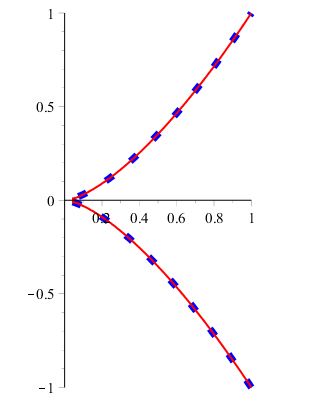
\includegraphics[scale=0.6]{Export/implicitplot1_2.png}
				\end{center}
			\end{column}
		\end{columns}
	\end{example}
\end{frame}

\begin{frame}
	\frametitle{Rosett}
	\begin{example}
		\begin{columns}[onlytextwidth]
			\begin{column}{0.5\textwidth}
\begin{semiverbatim}
> FindImplicitNotation(

\qquad t\^{}3*(t-1)\^{}3*(t+1)\^{}3,

\qquad t\^{}5*(t-1)\^{}2*(t+1)\^{}2, 

\qquad t, 150, true);


Elapsed Time: 1.266 s.
\end{semiverbatim}
\[
\begin{array}{l}
x^9-9x^8y+36x^7y^2-84x^6y^3+\\
+126x^5y^4-126x^4y^5+84x^3y^6-\\
-36x^2y^7+9xy^8-y^9+x^4y^3 = 0
\end{array}
\]
			\end{column}
			\begin{column}{0.5\textwidth}
				\begin{center}
					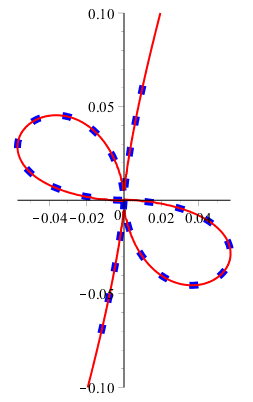
\includegraphics[scale=0.6]{Export/implicitplot6_2.png}
				\end{center}
			\end{column}
		\end{columns}
	\end{example}
\end{frame}




\section{Multiplicitetsföljder}

\subsection{Uppblåsningar}

\begin{frame}
	\frametitle{Plana algebraiska kurvor}
	\begin{center}
		\Large Multiplicitetsföljder
		
		Uppblåsningar
	\end{center}
\end{frame}

\begin{frame}
	\frametitle{Plan kurva med singularitet i origo}
	\begin{columns}[onlytextwidth]
		\begin{column}{0.5\textwidth}
			Betrakta den plana algebraiska kurvan $C(t)=(t^2,t^3+t^7)$. Denna ges implicit av ekvationen
			\[y^2-x^3-2x^5-x^7 = 0\]
			Vi ser att den har en singularitet i origo.
			
			\vspace{20pt}
			Hur kan vi göra den mjukare (eller enklare)?
		\end{column}
		\begin{column}{0.5\textwidth}
			\begin{center}
				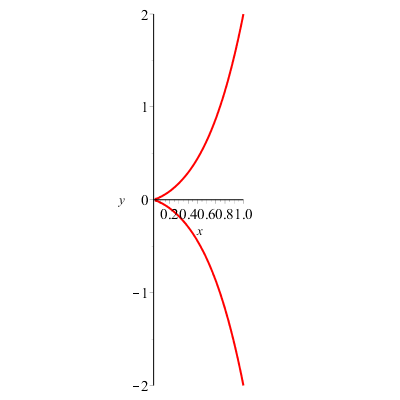
\includegraphics[scale=0.35]{Export/blowupex1_1.png}
			\end{center}
		\end{column}
	\end{columns}	
\end{frame}

\begin{frame}
	\frametitle{Projektion från en högre dimension}
	\begin{columns}[onlytextwidth]
		\begin{column}{0.4\textwidth}
			Enkelt att införa en tredje dimension med $z(t)=t$:
			\[C^*(t)=(t^2,t^3+t^7,t)\]
			
			Finns även tre projektioner utritade: 
			\[\left\{\begin{array}{l}
			P_x(t)=(x_p,y(t),z(t))\\
			P_y(t)=(x(t),y_p,z(t))\\
			P_z(t)=(x(t),y(t),z_p)
			\end{array}\right.\]
		\end{column}
		\begin{column}{0.6\textwidth}
			\begin{center}
				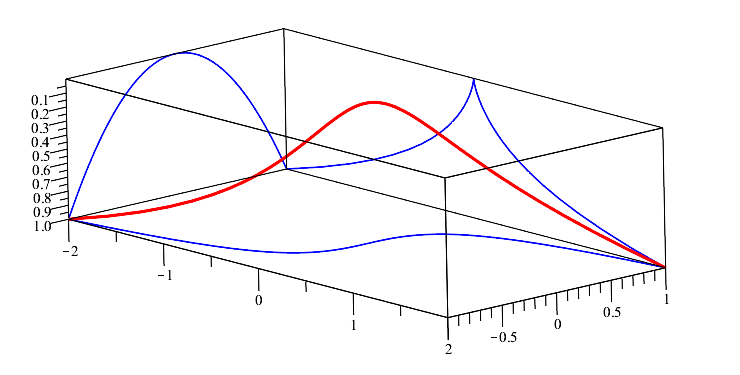
\includegraphics[scale=0.5]{Export/blowupex1_2.png}
			\end{center}
		\end{column}
	\end{columns}	
\end{frame}

\begin{frame}
	\frametitle{Implicit ekvation}
	Men hur gör vi med en algebraisk kurva som ges implicit av en polynomekvation $F(x,y)=0$?
	
	Istället kan vi införa en tredje dimension till kurvan genom att utanför singulariteten introducera $z=y/x, x \neq 0$.

	\begin{center}
		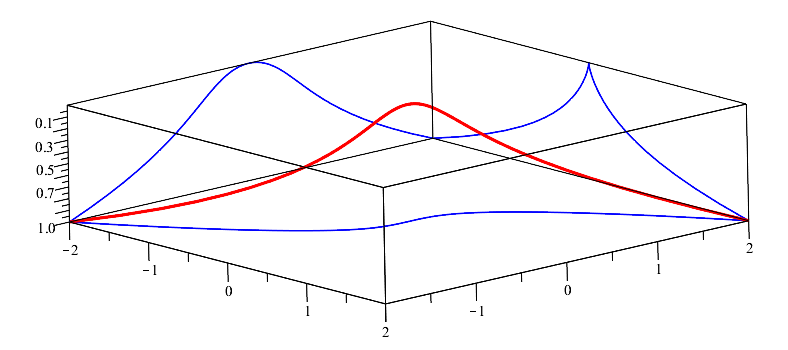
\includegraphics[scale=0.5]{Export/blowupex1_3.png}
	\end{center}
\end{frame}

\begin{frame}
	\frametitle{Agebraiska konsekvenser}
Eftersom vår ursprungliga kurva uppfyller $F(x,y)=0$ och den nya kurvan även uppfyller $z=y/x$, och därför $y=z\cdot x$, måste den nya kurvan således även uppfylla
\[F(x,z\cdot x)=0\]

I vårt exempel ger detta således:

\[
\begin{array}{c}
(z\cdot x)^2-x^3-2x^5-x^7 = x^2 \cdot \left(z^2-x-2x^3-x^5\right) = 0 \Longrightarrow\\[5pt]
\Longrightarrow (x=0) \vee (z^2-x-2x^3-x^5=0)\\
\end{array}
\]
\end{frame}

\begin{frame}
	\frametitle{Förenklad kurva}
	\begin{columns}[onlytextwidth]
		\begin{column}{0.5\textwidth}
			Vi får en ny kurva $C^*$, implicit givet av polynomekvationen \[F^*(x,z)=z^2-x-2x^3-x^5=0\] vilken är \emph{enklare} än den ursprungliga polynomekvationen $F(x,y)=0$.
			
			\vspace{20pt}
			Denna nya kurva $C^*$ motsvarar precis projektionen $P_y$ av vår tredimensionella kurva på XZ-planet.
		\end{column}
		\begin{column}{0.5\textwidth}
			\begin{center}
				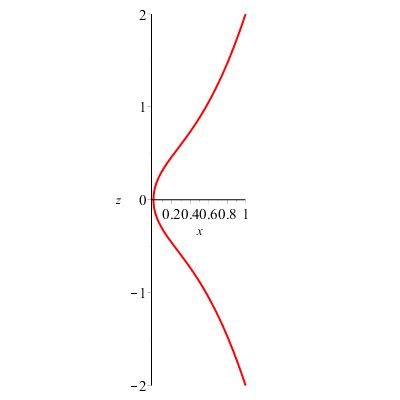
\includegraphics[scale=0.45]{Export/blowupex1_4.png}
			\end{center}
		\end{column}
	\end{columns}	
\end{frame}

\begin{frame}
	\frametitle{Uppblåsning}
\begin{Definition}
	En \textbf{uppblåsning} av en algebraisk plan singulär kurva $C$ som går genom origo, givet implicit genom polynomekvationen $F(x,y)=0$, är den algebraiska plana kurva $C^*$ som ges implicit av $F^*(x,y) = F(x,x\cdot y)/x^m=0$, där $m$ är \textbf{multipliciteten} av nollstället $x=0$ i $F(x,x\cdot y)$, dvs. det största heltal $m$ sådant att $x^m$ delar alla termer i $F(x,x\cdot y)$.
\end{Definition}
\uncover<2->{\begin{Corollary}
	För multipliciteten gäller att $m > 0$ om kurvan som ges av $F(x,y)=0$ går genom origo.
\end{Corollary}}
\end{frame}

\subsection{Multiplicitetsföljder}

\begin{frame}
	\frametitle{Plana algebraiska kurvor}
	\begin{center}
		\Large Multiplicitetsföljder
	\end{center}
\end{frame}

\begin{frame}
	\frametitle{Serie av uppblåsningar}
Låt oss kalla uppblåsningsoperatorn definierad ovan för $B$ (för ``Blow-Up''), där $F(x,y)$ blåses upp till $F^*(x,y)$ och $m$ är den implicit genererade multipliciteten i operationen:

\[F \overset{B}{\underset{m}{\longrightarrow}} F^*\]

Anta att vi har en serie uppblåsningar:

\[
F(x,y) \overset{B}{\underset{m_1}{\longrightarrow}} F_1(x,y) \overset{B}{\underset{m_2}{\longrightarrow}} \ldots \overset{B}{\underset{m_n}{\longrightarrow}} F_n(x,y) \overset{B}{\underset{m_{n+1}}{\longrightarrow}} \ldots
\]

Denna serie kan bara fortgå så länge $F_i(x,y)$ är singulär i origo. Hur länge är det? 
\end{frame}

\begin{frame}
	\frametitle{Oändligt exempel}
	\begin{example}
		Låt oss betrakta $F(x,y)=y^2-xy$:
		
		\[
		(y^2-xy) \overset{B}{\underset{2}{\longrightarrow}} (y^2-y) \overset{B}{\underset{1}{\longrightarrow}} (xy^2-y) \overset{B}{\underset{1}{\longrightarrow}} (x^2y^2-y) 		
		\overset{B}{\underset{1}{\longrightarrow}}\]
		\[\overset{B}{\underset{1}{\longrightarrow}} (x^3y^2-y) \overset{B}{\underset{1}{\longrightarrow}} \ldots\]
		
		Multiplicitetsföljden blir $2,1,1,1,1,\ldots$, i all oändlighet. Anledningen till detta är att alla termer innehåller $y$ som alltid genererar en faktor $x$ för varje uppblåsning.
	\end{example}
\end{frame}

\begin{frame}
	\frametitle{Ändliga multiplicitetsföljder}
	\begin{Theorem}
		Om $F(x,y)\in \mathbb{C}[x,y]$ är singulär i origo och är summan av ett polynom $G(x,y)=y\cdot H(x,y)$, vilket har minst ett $y$ i varje term, och ett polynom $p(x) \neq 0$ som bara har termer bestående av potenser av $x$, så är multiplicitetsföljden av $F(x,y)$ en ändlig serie av icke strikt avtagande heltal.
	\end{Theorem}

	\uncover<2->{Översikt av bevis: (1/6)}
	\begin{enumerate}
		\item<3->$n=\mathbf{o}(p)$
		\item<4->$F(x,y)=G(x,y)+x^nq(x)$, $q(0)\neq 0$
		\item<5->$
		G(x,y)+x^nq(x) \overset{B}{\underset{m_1}{\longrightarrow}} G_1(x,y)+x^{n-m_1}q(x) \overset{B}{\underset{m_2}{\longrightarrow}} \ldots \overset{B}{\underset{m_i}{\longrightarrow}}
		G_i(x,y)+x^{n-\sum_{j=1}^{i}m_j}q(x) \overset{B}{\underset{m_{i+1}}{\longrightarrow}} \ldots$
	\end{enumerate}
\end{frame}

\begin{frame}
	\frametitle{Ändliga multiplicitetsföljder}
	\begin{Theorem}
		Om $F(x,y)\in \mathbb{C}[x,y]$ är singulär i origo och är summan av ett polynom $G(x,y)=y\cdot H(x,y)$, vilket har minst ett $y$ i varje term, och ett polynom $p(x) \neq 0$ som bara har termer bestående av potenser av $x$, så är multiplicitetsföljden av $F(x,y)$ en ändlig serie av icke strikt avtagande heltal.
	\end{Theorem}
			
	Översikt av bevis: (2/6)
	\begin{enumerate}
		\setcounter{enumi}{3}
		\item För $G_i(x,y)$ gäller följande:
		\begin{enumerate}
			\item<2-> Samma antal termer.
			\item<3-> $G_i(0,0)=0$
		\end{enumerate}
		\item<4-> $\sum_{j=1}^{i}m_j<n \Longrightarrow \left.G_i(x,y)+x^{n-\sum_{j=1}^{i}m_j}q(x) \middle|\raisebox{-0.5 em}{\scriptsize(0,0)}=0\right.$
	\end{enumerate}
\end{frame}

\begin{frame}
	\frametitle{Ändliga multiplicitetsföljder}
	\begin{Theorem}
		Om $F(x,y)\in \mathbb{C}[x,y]$ är singulär i origo och är summan av ett polynom $G(x,y)=y\cdot H(x,y)$, vilket har minst ett $y$ i varje term, och ett polynom $p(x) \neq 0$ som bara har termer bestående av potenser av $x$, så är multiplicitetsföljden av $F(x,y)$ en ändlig serie av icke strikt avtagande heltal.
	\end{Theorem}
	
	Översikt av bevis: (3/6)
	\begin{enumerate}
		\setcounter{enumi}{5}
		\item $m_{i+1}>0$
		\item<2-> Sekvensen måste få ett stopp efter $N$ steg: $\sum_{j=1}^{N}m_j=n$
		\item<3-> Sista uppblåsningen blir $G_N(x,y)+q(x)$
	\end{enumerate}
\end{frame}

\begin{frame}
	\frametitle{Ändliga multiplicitetsföljder}
	\begin{Theorem}
		Om $F(x,y)\in \mathbb{C}[x,y]$ är singulär i origo och är summan av ett polynom $G(x,y)=y\cdot H(x,y)$, vilket har minst ett $y$ i varje term, och ett polynom $p(x) \neq 0$ som bara har termer bestående av potenser av $x$, så är multiplicitetsföljden av $F(x,y)$ en ändlig serie av icke strikt avtagande heltal.
	\end{Theorem}
	
	Översikt av bevis: (4/6)
	\begin{enumerate}
		\setcounter{enumi}{8}
		\item $F(x,y) = \sum_{i\in I} p_i(x)y^i = \sum_{i\in I} x^{n_i}q_i(x)y^i$
		\item<2-> $F(x,y) \overset{B}{\underset{m_1}{\longrightarrow}} \frac{F(x,x\cdot y)}{x^{m_1}}=\sum_{i\in I} x^{n_i+i-m_1}q_i(x)y^i$
		\item<3-> $m_1=\min(\left\{n_i+i\right\}_{i\in I})$
		\item<4-> $\exists i_1:n_{i_1}+i_1-m_1=0$
	\end{enumerate}
\end{frame}

\begin{frame}
	\frametitle{Ändliga multiplicitetsföljder}
	\begin{Theorem}
		Om $F(x,y)\in \mathbb{C}[x,y]$ är singulär i origo och är summan av ett polynom $G(x,y)=y\cdot H(x,y)$, vilket har minst ett $y$ i varje term, och ett polynom $p(x) \neq 0$ som bara har termer bestående av potenser av $x$, så är multiplicitetsföljden av $F(x,y)$ en ändlig serie av icke strikt avtagande heltal.
	\end{Theorem}
	
	Översikt av bevis: (5/6)
	\begin{enumerate}
		\setcounter{enumi}{12}
		\item $\ldots \overset{B}{\underset{m_2}{\longrightarrow}} \sum_{i\in I} x^{n_i+(i-m_1)+(i-m_2)}q_i(x)y^i$
		\item<2-> $m_2\leq i_1$
		\item<3-> $i_1=m_1-n_{i_1}\leq m_1 \Longrightarrow m_2\leq m_1$
		\item<4-> Antag $m_1\geq m_2 \geq \ldots \geq m_k, k \geq 2$
	\end{enumerate}
\end{frame}

\begin{frame}
	\frametitle{Ändliga multiplicitetsföljder}
	\begin{Theorem}
		Om $F(x,y)\in \mathbb{C}[x,y]$ är singulär i origo och är summan av ett polynom $G(x,y)=y\cdot H(x,y)$, vilket har minst ett $y$ i varje term, och ett polynom $p(x) \neq 0$ som bara har termer bestående av potenser av $x$, så är multiplicitetsföljden av $F(x,y)$ en ändlig serie av icke strikt avtagande heltal.
	\end{Theorem}
	
	Översikt av bevis: (6/6)
	\begin{enumerate}
		\setcounter{enumi}{16}
		\item $\ldots \overset{B}{\underset{m_{k+1}}{\longrightarrow}} \sum_{i\in I} x^{n_i+\sum_{j=1}^{k} (i-m_j) + (i-m_{k+1})}q_i(x)y^i$
		\item<2-> Om nu $m_{k+1}>m_k$ ser vi att vi hade kunnat subtrahera ytterligare från exponenten i tidigare skede (i exponentens $(i-m_k)$-term) genom att göra $m_k$ större.
		\qed
	\end{enumerate}
\end{frame}

\begin{frame}
	\frametitle{}
\begin{Corollary}
	Givet $F(x,y)=y\cdot H(x,y)+p(x)$ och dess multiplicitetsföljd $\left\{m_i\right\}$, gäller att $\mathbf{o}(p)=\sum m_i$.
\end{Corollary}

\vspace{20pt}
\uncover<2->{
	\mbox{
\scriptsize Not: Ovanstående håller även i fallet då $p(x)=0$, om man definierar $\mathbf{o}(0)=\infty$.}}

\vspace{20pt}
\uncover<3->{
\begin{Corollary}
	Om $F(x,y)\in \mathbb{C}[x,y]$ är ett irreducibelt polynom som är singulärt i origo, så är multiplicitetsföljden av $F(x,y)$ en ändlig serie av icke strikt avtagande heltal.
\end{Corollary}
}
\end{frame}

\begin{frame}
	\frametitle{\texttt{MultiplicitySequenceXY()}}
	
	\begin{semiverbatim}
		MultiplicitySequenceXY := proc(F, XVariable, YVariable)
	\end{semiverbatim}
	
	\begin{enumerate}
		\item<1-> Algoritm som beräknar multiplicitetsföljden av en algebraisk kurva givet på formen $F(x, y) = 0$, där $F \in \mathbb{C}\left[x, y\right]$.
		
		\item<2-> Maple-kod finns i \texttt{https://github.com/PeterWaher/\\
			\qquad Algebraiska\_kurvor/blob/master/\\
			\qquad multiplicitetsfoljder.mw}
		
		\item<3-> Text-version finns i
		\texttt{https://github.com/PeterWaher/\\
			\qquad Algebraiska\_kurvor/blob/master/Functions/\\
			\qquad MultiplicitySequenceXY.txt} 
	\end{enumerate}
\end{frame}

\begin{frame}
	\frametitle{Exempel 1/2}
	\begin{example}
I detta exempel beräknas multiplicitetsföljden för $y^2 - x^5 = 0$:

\begin{semiverbatim}
> MultiplicitySequenceXY(y\^{}2-x\^{}5,x,y)
\end{semiverbatim}
\[\left[2, 2, 1\right]\]
	\end{example}
\end{frame}

\begin{frame}
	\frametitle{Exempel 2/2}
	\begin{example}
		Vill vi se de successiva uppblåsningarna gör vi som följer:
		
		\begin{semiverbatim}
			> MultiplicitySequenceXY(y\^{}2-x\^{}5,x,y,true)
		\end{semiverbatim}
		\[[2,-x^3+y^2]\]
		\[[2,y^2-x]\]
		\[[1,xy^2-1]\]
		\[[0,x^3y^2-1]\]
		\[\left[2, 2, 1\right]\]
	\end{example}
\end{frame}



\subsection{Funktionsfamiljer}

\begin{frame}
	\frametitle{Plana algebraiska kurvor}
	\begin{center}
		\Large Multiplicitetsföljder
		
		Funktionsfamiljer
	\end{center}
\end{frame}

\begin{frame}
	\frametitle{Funktionsfamiljer}
	Givet en multiplicitetsföljd $\left\{m_i\right\}$, hur ser funktionerna $F(x,y)$ ut som har motsvarande multiplicitetsföljd?
	
	\uncover<2->{
	Algoritm för att beräkna familj av funktioner som har given multiplicitetsföljd:}
	
	\begin{enumerate}
		\item<3-> $s=\sum_{i=1}^{n} m_i$
		\item<4-> $F(x,y)=\left(\sum_{i=1}^{m_1}\left(\sum_{j=0}^{s-i} a_{i,j} x^j y^i\right)\right)-x^s$
		\item<5-> Vi inte behöver ta med termer innehållande faktorer av $y$ med högre potens än $m_1$.
		\item<6-> Utför serie uppblåsningar: Avgör vilka $a_{i,j}=0$.
		\item<7-> Utför ny serie uppblåsningar: Avgör vilka $a_{i,j} \neq 0$.
		\item<8-> Beräkna ``enklaste'' lösningen.
		\item<9-> Om motsägelser uppstår, rapporteras fel.
	\end{enumerate}
\end{frame}

\begin{frame}
	\frametitle{Hittas alltid en lösning?}
	
	Finns alltid en lösning?
	
	\begin{enumerate}
		\item<2-> Lösning ej garanterad.
		
		\item<3-> Inkonsistenta samband mellan koefficienter.
		
		\item<4-> Vissa val av kombinationer kan ge annorlunda multiplicitetsföljd.
		
		\item<5-> ``Enklaste'' lösningen inte nödvändigtvis \emph{irreducibel}.
		
		\item<6-> Inga fel eller avbrott rapporteras efter en genomgång av alla multiplicitetsföljder upp till multiplicitetssumma 30. Det finns 28628 sådana multiplicitetsföljder.
	\end{enumerate}
\end{frame}

\begin{frame}
	\frametitle{\texttt{FindFunctionXYFromMultiplicitySequence()}}
	
	\begin{semiverbatim}
		FindFunctionXYFromMultiplicitySequence := 

\qquad proc(Sequence, CalcFamily)
	\end{semiverbatim}
	
	\begin{enumerate}
		\item<1-> Algoritm som beräknar fram en funktion $F(x,y)$, $F(x, y) \in \mathbb{C}\left[x, y\right]$ vars multiplicitetsföljd är given i anropet.
		
		\item<2-> Maple-kod finns i \texttt{https://github.com/PeterWaher/\\
			\qquad Algebraiska\_kurvor/blob/master/\\
			\qquad multiplicitetsfoljder.mw}
		
		\item<3-> Text-version finns i
		\texttt{https://github.com/PeterWaher/\\
			\qquad Algebraiska\_kurvor/blob/master/Functions/\\
			\qquad FindFunctionXYFromMultiplicitySequence.txt} 
	\end{enumerate}
\end{frame}

\begin{frame}
	\frametitle{Exempel}
	\begin{example}
		I följande exempel beräknas en familj av polynom $F(x, y) \in \mathbb{C}[x, y]$ sådana att kurvorna $F(x, y) = 0$ har multiplicitetsföljden 2, 2, 1.
		
		\begin{semiverbatim}
			> FindFunctionXYFromMultiplicitySequence(

\qquad [2,2,1], true)
		\end{semiverbatim}
\[
\begin{array}{l}
\left[-x^5+y^2,\right.\\
x^4ya_5+x^3y^2a_9-x^5+x^3ya_4+x^2y^2a_8+x^2ya_3+xy^2a_7+y^2a_6,\\
\left.a_6 \neq 0\right]\\
\end{array}
\]
	\end{example}
\end{frame}



\subsection{Komplexitet}

\begin{frame}
	\frametitle{Plana algebraiska kurvor}
	\begin{center}
		\Large Multiplicitetsföljder
		
		Komplexitet
	\end{center}
\end{frame}

\begin{frame}
	\frametitle{Antal multiplicitetsföljder}
När vi börjar undersöka hur väl beräkningen av funktionsfamiljer från multiplicitetsföljderna går, ser vi att en intressant talföljd $\left\{N_i\right\}$ uppstår, där $N_i$ är antalet multiplicitetsföljder som finns vars multipliciteter summerar till $i$.

\begin{center}
	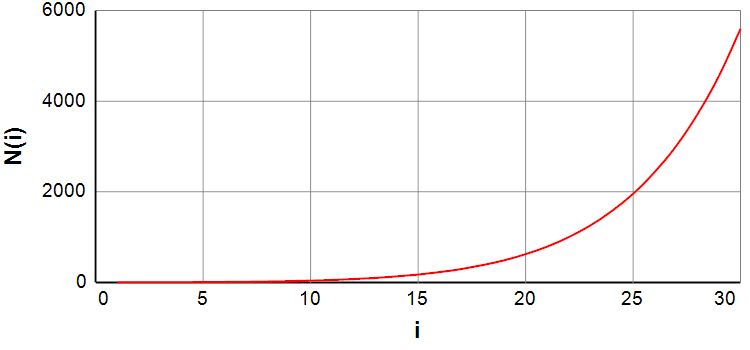
\includegraphics[scale=0.5]{Export/Complexity1.png}
\end{center}
\end{frame}

\begin{frame}
	\frametitle{Rekursiv definition}
	Är talföljden asymptotisk och växer på ett förutbestämt sätt, liknande
	exempelvis \emph{Fibonacci}-följden?
	
	\[
	\begin{array}{rcl}
	N_i & \equiv & N_{i,i} \\[5pt]
	N_{i,j} & = & \left\{
	\begin{array}{ll}
	0 & , i < 0 \vee j \leq 0\\[5pt]
	1 & ,i=0 \wedge j > 0\\[5pt]
	\displaystyle\sum_{k=1}^{\min(i,j)}N_{i-k,k} & ,i>0 \wedge j>0\\
	\end{array}
	\right.\\
	\end{array}
	\]
\end{frame}

\begin{frame}
	\frametitle{Polynomial tillväxt?}
	{
	\Large
	Växer följden som ett polynom?
	}
	
	\vspace{20pt}
	Försöker vi med hjälp av minsta kvadratmetoden passa in polynom på denna kurva kommer vi inte hitta någon som passar. Istället ser vi hur termerna i polynomen alternerar mellan positiva och negativa, i takt med att vi försöker med högre och högre grader, något som kan indikera en exponentiell tillväxt.
\end{frame}

\begin{frame}
	\frametitle{Exponentiell tillväxt?}
	{
		\Large
		Växer följden exponentiellt?
	}
	
	\vspace{20pt}
	Empiriskt ser $\ln(N_i)^{3/2}$ intressant ut:
	\begin{center}
		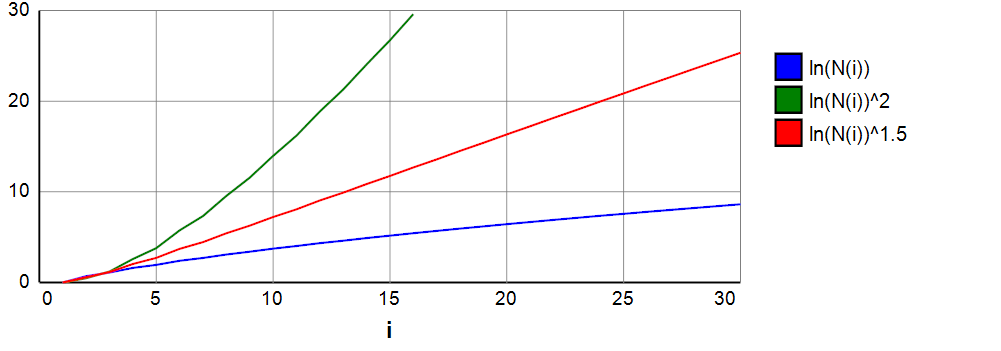
\includegraphics[scale=0.5]{Export/Complexity2.png}
	\end{center}
\end{frame}

\begin{frame}
	\frametitle{Första ansats}
\[\ln(N_i)^E \approx a+b\cdot i \Longleftrightarrow N_i \approx e^{(a+b\cdot i)^{\frac{1}{E}}} \]

$SE(E)$ ger minstakvadratenfelet, $a,b$ fås genom linjär regression.

\[
\begin{array}{cc}
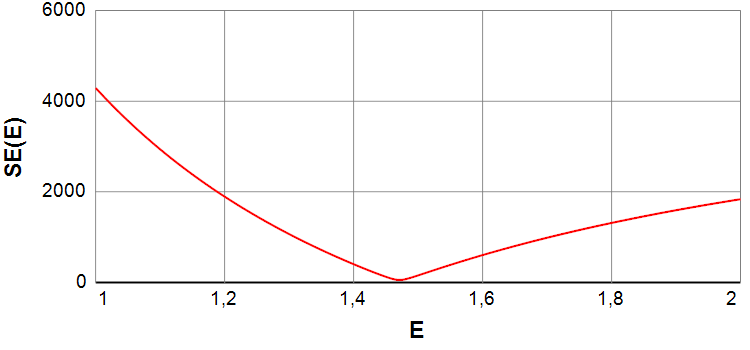
\includegraphics[scale=0.35]{Export/Complexity3.png}
&
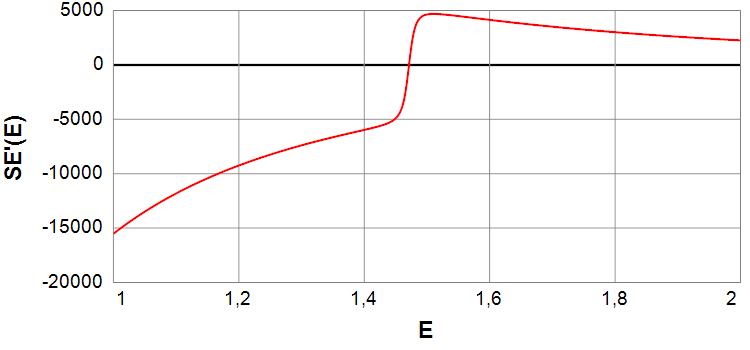
\includegraphics[scale=0.35]{Export/Complexity4.png}\\
\end{array}
\]
\[_{E=1.47126405685409, \:a=-1.34861467338489, \:b=0.839860447173521}\]

\end{frame}

\begin{frame}
	\frametitle{Resultat}
Vi kan nu jämföra vår modell med det uppmätta värdena, för att se hur väl de stämmer överens. Till synes ganska väl, även om det inte är perfekt.
\[
\begin{array}{cc}
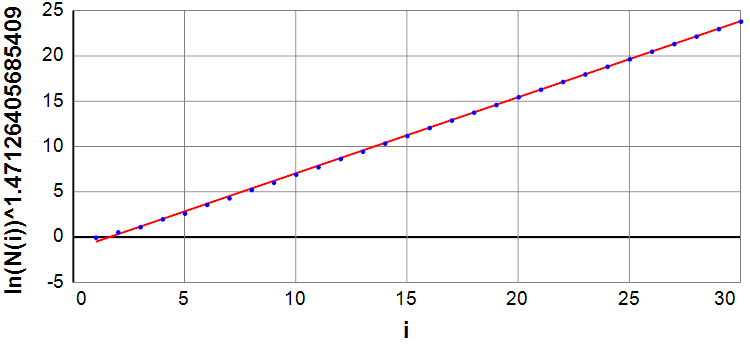
\includegraphics[scale=0.35]{Export/Complexity5.png}
&
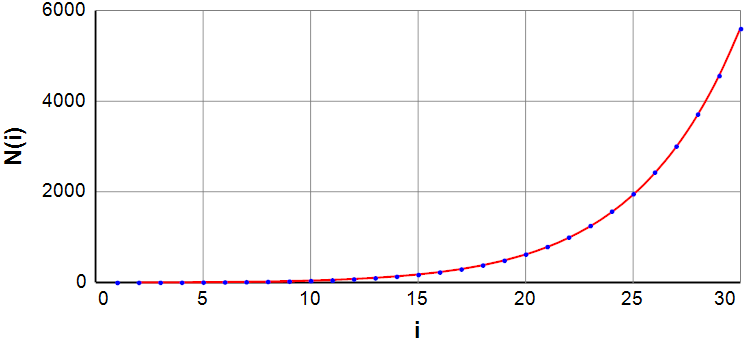
\includegraphics[scale=0.35]{Export/Complexity6.png}\\
\end{array}
\]
\end{frame}

\begin{frame}
	\frametitle{Modellen ser inte ut att hålla}
Visar vi istället skillnaden mellan uppmätt och uppskattat i fallet med $\ln(N_i)$ och felet mellan uppmätt och uppskattat i fallet med $N_i$ ser vi att vår uppskattning antagligen inte kommer att hålla:
\[
\begin{array}{cc}
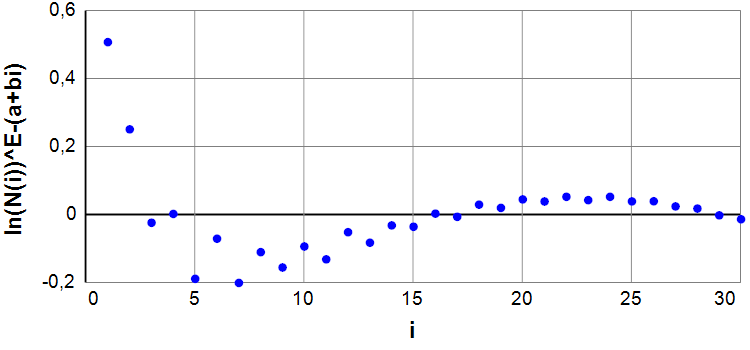
\includegraphics[scale=0.35]{Export/Complexity7.png}
&
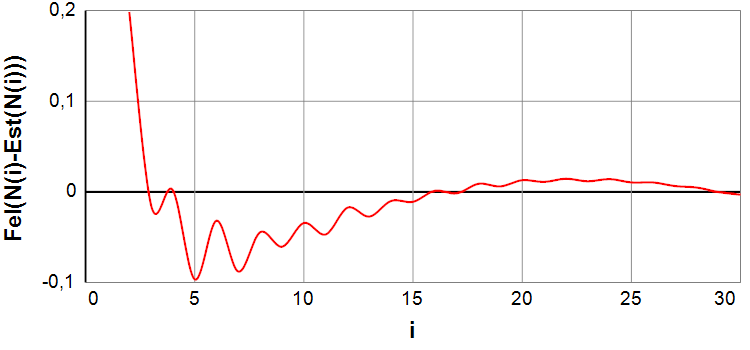
\includegraphics[scale=0.35]{Export/Complexity8.png}\\
\end{array}
\]
\end{frame}

\begin{frame}
	\frametitle{Modellen håller inte}
	Specialkod i Maple beräknar $N_i$ upp till $i=100$:
\[
\begin{array}{cc}
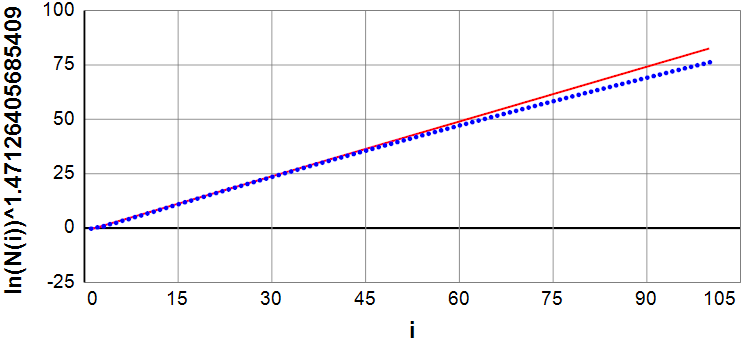
\includegraphics[scale=0.35]{Export/Complexity9.png}
&
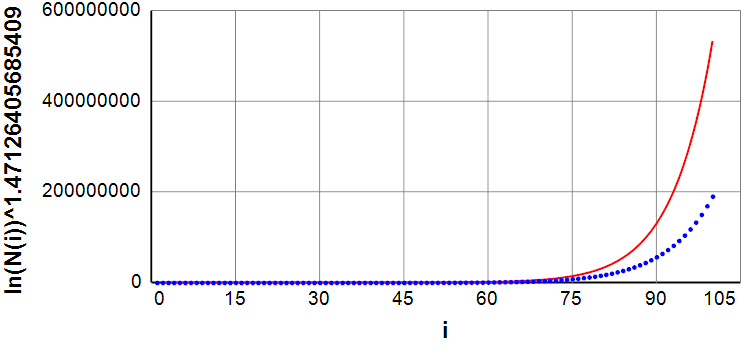
\includegraphics[scale=0.35]{Export/Complexity10.png}\\
\end{array}
\]

Det som är den bästa linjen på intervallet $[1,30]$ är inte den bästa linjen på intervallet $[1,100]$.
\end{frame}

\begin{frame}
	\frametitle{Är följden asymptotisk mot en geometrisk serie?}
	Kommer $N_i$ gå asymptotiskt mot en geometrisk serie $N_i \rightarrow c\cdot P^i$? Eller kommer $N_{i+1}/N_i \rightarrow 1$ då $i \rightarrow \infty$? Om $Q_i=N_i/N_{i-1}$, kommer då $Q_i \rightarrow P$ för något $P>1$?

\begin{center}
	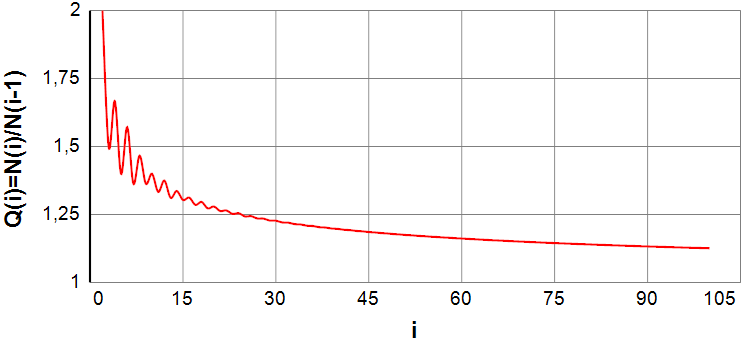
\includegraphics[scale=0.5]{Export/Complexity11.png}
\end{center}
\end{frame}

\begin{frame}
	\frametitle{$Q_i$ verkar gå mot 1}
	Genom att utnyttja ett specialprogram skrivet i C\# har vi lyckats beräkna $N_i$ och $Q_i$ upp till $i=10000$.
	
	\begin{center}
		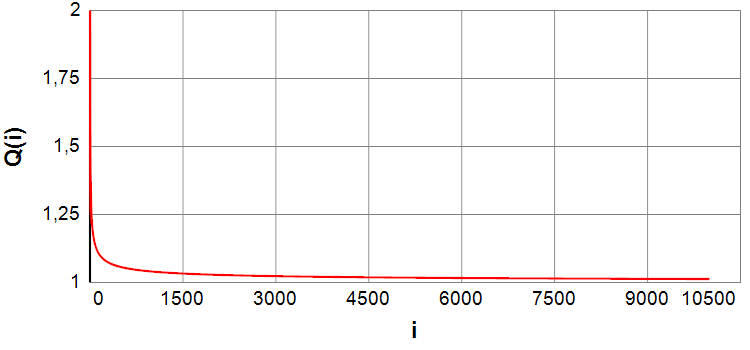
\includegraphics[scale=0.5]{Export/Complexity12.png}
	\end{center}
	
	{\scriptsize
	\[
	\begin{array}{rcl}
	N_{10000} & = & 361672513256362939888204718909536954950160303393156\ldots\\
	& & \ldots504220818686058879525687540664205923105560529069\ldots\\
	& & \ldots16435144\\
	Q_{10000} & = & 1.0128073565554...
	\end{array}
	\]
	}
\end{frame}

\begin{frame}
	\frametitle{$Q_i$ en invers?}
	{
		\Large
		Avtar $Q_i$ som en invers av något?
	}
	
	\vspace{20pt}
	Empiriskt ser $1/(Q_i-1)^2$ intressant ut:
	\begin{center}
		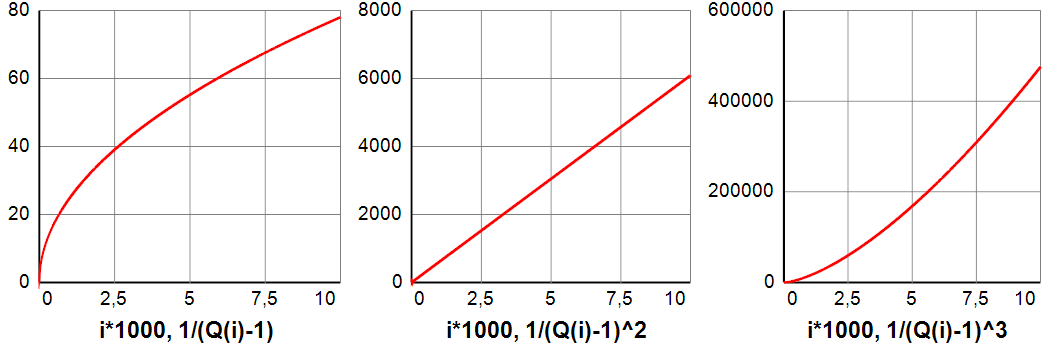
\includegraphics[scale=0.5]{Export/Complexity13.png}
	\end{center}
\end{frame}

\begin{frame}
	\frametitle{Sökning efter exponent}
	$SEQ(E)$ ger minstakvadratenfelet mellan bästa linjen och $\frac{1}{(Q_i-1)^E}$.
	
\[
\begin{array}{cc}
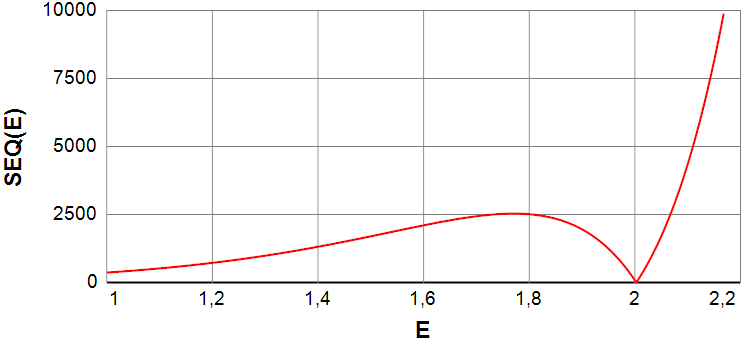
\includegraphics[scale=0.35]{Export/Complexity14.png}
&
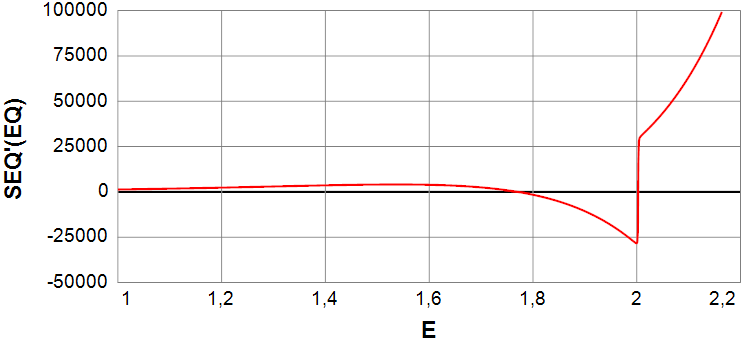
\includegraphics[scale=0.35]{Export/Complexity15.png}\\
\end{array}
\]
\[E_{[1,10000]} = 2.00264350576171\]
\end{frame}

\begin{frame}
	\frametitle{Hur bra är uppskattningen av exponenten?}
	Hur mycket beror vårt resultat på intervallet vi valt ($Q_1-Q_{10000}$)?

	\begin{center}
	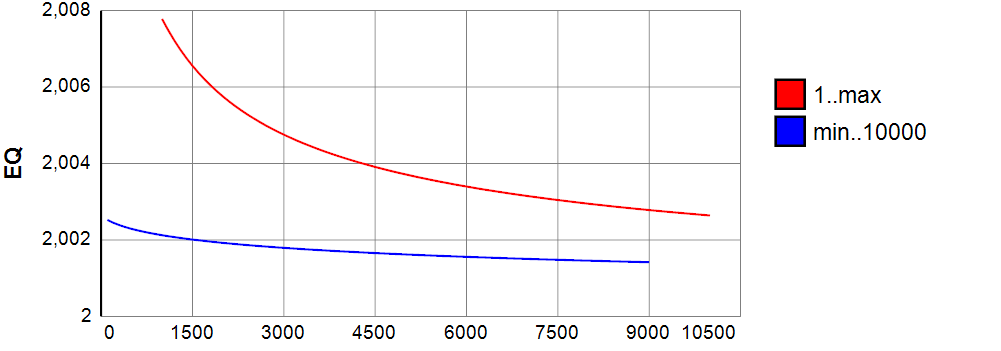
\includegraphics[scale=0.5]{Export/Complexity16.png}
	\end{center}
	\[E_{[9000,10000]} = 2.00142039633785\]
\end{frame}

\begin{frame}
	\frametitle{Andra ansats}
Från vår empiriska studie över antalet multiplicitetsföljder $N_i$, och dess förhållanden $Q_i=N_i/N_{i-1}$, är det således inte helt orimligt att göra följande antagande angående $Q_i$'s asymptotiska beteende:

\[\frac{1}{\left(Q_i-1\right)^2} \sim a+b\cdot i \text{, (då $i \rightarrow \infty$)}\]
\[\Longleftrightarrow \]
\[Q_i \sim 1+\frac{1}{\sqrt{a+b\cdot i}}\text{, (då $i \rightarrow \infty$)} \]
\end{frame}

\begin{frame}
	\frametitle{Nelder-Mead}
		
	\[f_\mathbf{v}(i)=v_0+\frac{v_1}{\sqrt{v_2+v_3 i+v_4 i^2+v_5 i^3+v_6 i^4+v_7 i^5+v_8 i^6+v_9 i^7}}\]
	
	Med hjälp av \emph{Nelder-Mead's algoritm} optimerar vi så att felet mellan $f_\mathbf{v}(i)$ och $Q_i$ blir så litet som möjligt:
	\[\begin{array}{l}
	\text{NM}(f_\mathbf{v},\left\{1,1,1,1,0,0,0,0,0,0\right\})=\\
	\qquad\left\{1, 1.27124055101012, 1, 1, 0; 0; 0; 0; 0; 0\right\}\end{array}\]
	
	Vi har således fått en uppskattning av $Q_i$:
	\[Q_i \approx 1+\frac{1.27124055101012}{\sqrt{1+i}} \]	
\end{frame}

\begin{frame}
	\frametitle{Resultat}
Vi kan rita ut $Q_i$ tillsammans med sin uppskattning, och ser att de verkar stämma överens ganska bra:

\begin{center}
	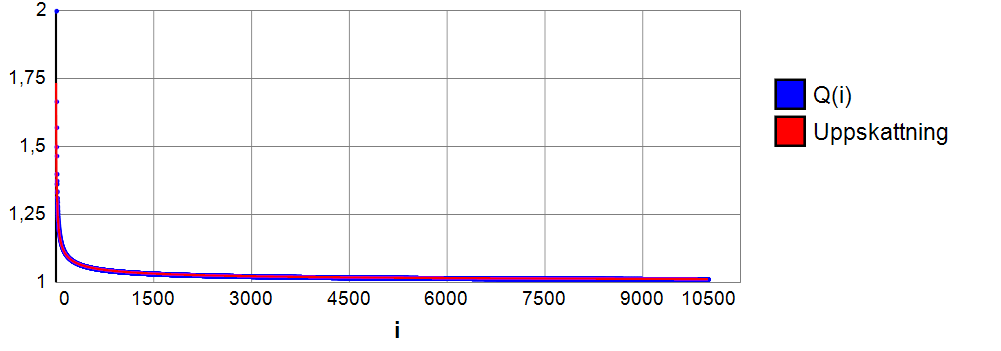
\includegraphics[scale=0.5]{Export/Complexity17.png}
\end{center}
\end{frame}

\begin{frame}
	\frametitle{Feluppskattning}
Ännu bättre ser vi att de stämmer överens om vi ritar ut felet mellan $Q_i$ och dess uppskattning, $\text{Err}_Q(i)$:

\begin{center}
	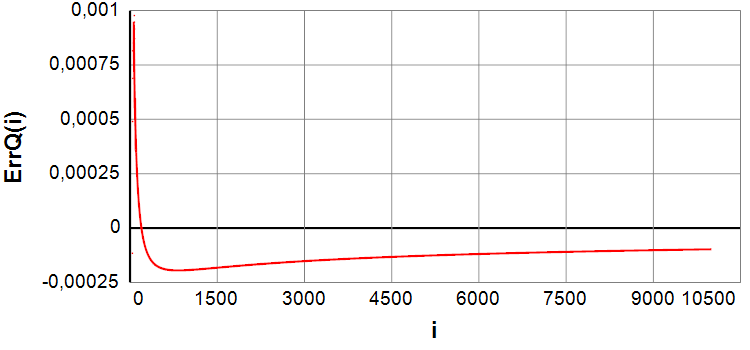
\includegraphics[scale=0.5]{Export/Complexity18.png}
\end{center}
\end{frame}

\begin{frame}
	\frametitle{Slutsats}
Inte bara är felet litet, det verkar gå mot noll då $i$ växer, utan tendens att divergera. Vi kan således dra slutsatsen att $N_i$ \emph{inte} växer exponentiellt, i motsats till vad vi antog i början. Istället verkar den växa i enlighet med:
\[N_i = \prod_{k=1}^{i} Q_i = \prod_{k=1}^{i} \left(1+\frac{1.27124055101012}{\sqrt{1+k}}+\text{Err}_Q(k)\right) \]
där $\text{Err}_Q(k)$ verkar gå mot 0 då $k \rightarrow \infty$.
\end{frame}

\begin{frame}
	\frametitle{Propagerat fel}
Dock har felet i uppskattningen av $Q_i$ väldigt stor påverkan på den multiplikativa uppskattningen av $N_i$, som kan ses av följande graf som är förhållandet mellan $N_i$ och
\[N^-_i=\prod_{k=1}^{i} \left(1+\frac{1.27124055101012}{\sqrt{1+k}}\right)\]

\begin{center}
	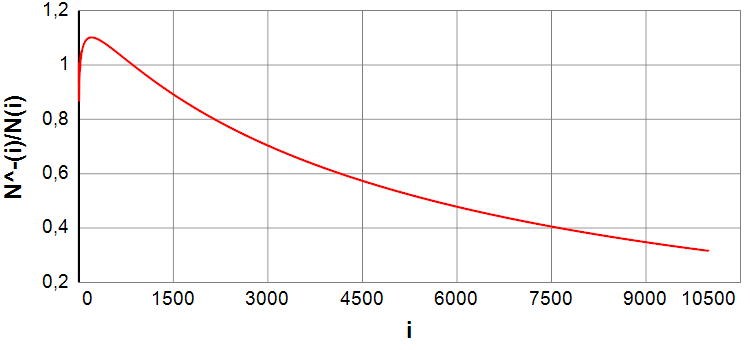
\includegraphics[scale=0.5]{Export/Complexity19.png}
\end{center}
\end{frame}

\begin{frame}
	\frametitle{Begränsning}
Vi ser att efter $i=856$ gäller att $N_i>N^-_i$. Vi vet också att $\text{Err}_Q(856) \approx -0.000194294156604657$, och att $\text{Err}_Q(i)$ är svagt växande därefter.
\[N^+_i = N_{856} \cdot \prod_{k=1}^{i} \left(1+\frac{1.27124055101012}{\sqrt{1+k}}-\text{Err}_Q(856)\right), i\geq 856 \]
\begin{center}
	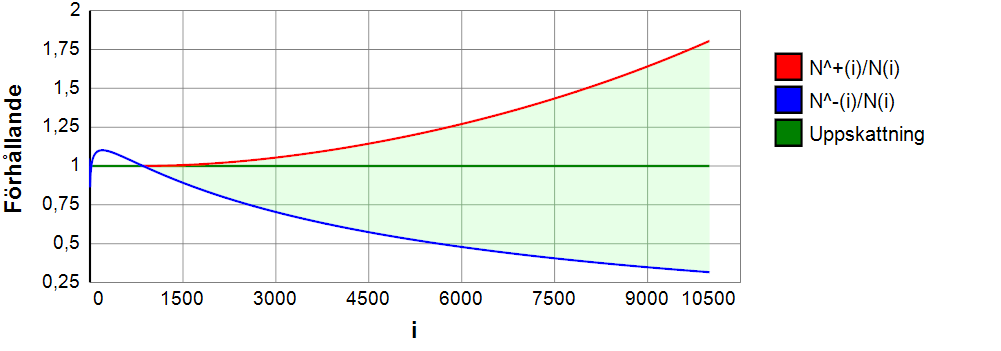
\includegraphics[scale=0.5]{Export/Complexity20.png}
\end{center}
\end{frame}

\begin{frame}
	\frametitle{Tack}
	
	\begin{center}
		\Large Tack för din tid
		
		\vspace{20pt}
		
		\normalsize
Också ett stort tack till Rikard Bögvad, och speciellt Ralf Fröberg, för all den tålamod och goda vilja de visat under loppet av detta arbete. Men sådan är naturen hos $\mathfrak{L}_2$-arbeten som detta.
	\end{center}
\end{frame}



\end{document}